\chapter{Dise\~no, Implementaci\'on y Prueba}
En este cap\'itulo se presentan los detalles de dise\~no e implementaci\'on del sistema, empezando con un simple diagrama de paquetes general hasta llegar a explicar los detalles internos de su desarrollo.

\section{Dise\~no General del Sistema}
Como dise\~no general del sistema se denota la agrupaci\'on de los componentes en paquetes seg\'un su comportamiento y funcionalidad.\\

El sistema se divide en 4 paquetes b\'asicos:
\begin{itemize}
	\item \textit{jtlc.core}: contiene los componentes que forman la l\'ogica del sistema, los modelos (Experimento, Muestra y Pico), las unidades que permiten llevar a cabo el proceso (Procesado de im\'agenes y An\'alisis de datos), la generaci\'on de reportes y el almacenamiento en disco de los experimentos realizados.
	\item \textit{jtlc.assets}: engloba los recursos b\'asicos del sistema, los elementos gr\'aficos, las plantillas de reportes, los documentos de informaci\'on al usuario y los paquetes de idiomas.
	\item \textit{jtlc.view}: agrupa todos los componentes que forman las diferentes interfaces gr\'aficas, la vista principal, los cuadros de di\'alogo, los paneles de cada etapa del proceso y los componentes personalizados. Tambi\'en contiene los diferentes DTO (Data Transfer Object) que permiten el intercambio de informaci\'on entre los componentes gr\'aficos y los controladores.
	\item \textit{jtlc.main}: incluye los componentes principales del sistema, las estructuras globales que se utilizan a lo largo de todo el sistema, el controlador principal que maneja las vistas y la tarea que se encarga de iniciar la aplicaci\'on.
\end{itemize}

En el siguiente diagrama de paquetes \cite{uml} (figura \ref{fig:disenoPaquetes}) se detallan los paquetes que componen el sistema y su asociaci\'on.\\
\begin{figure}[H]
	\centering
	\vspace{-0.5cm}
	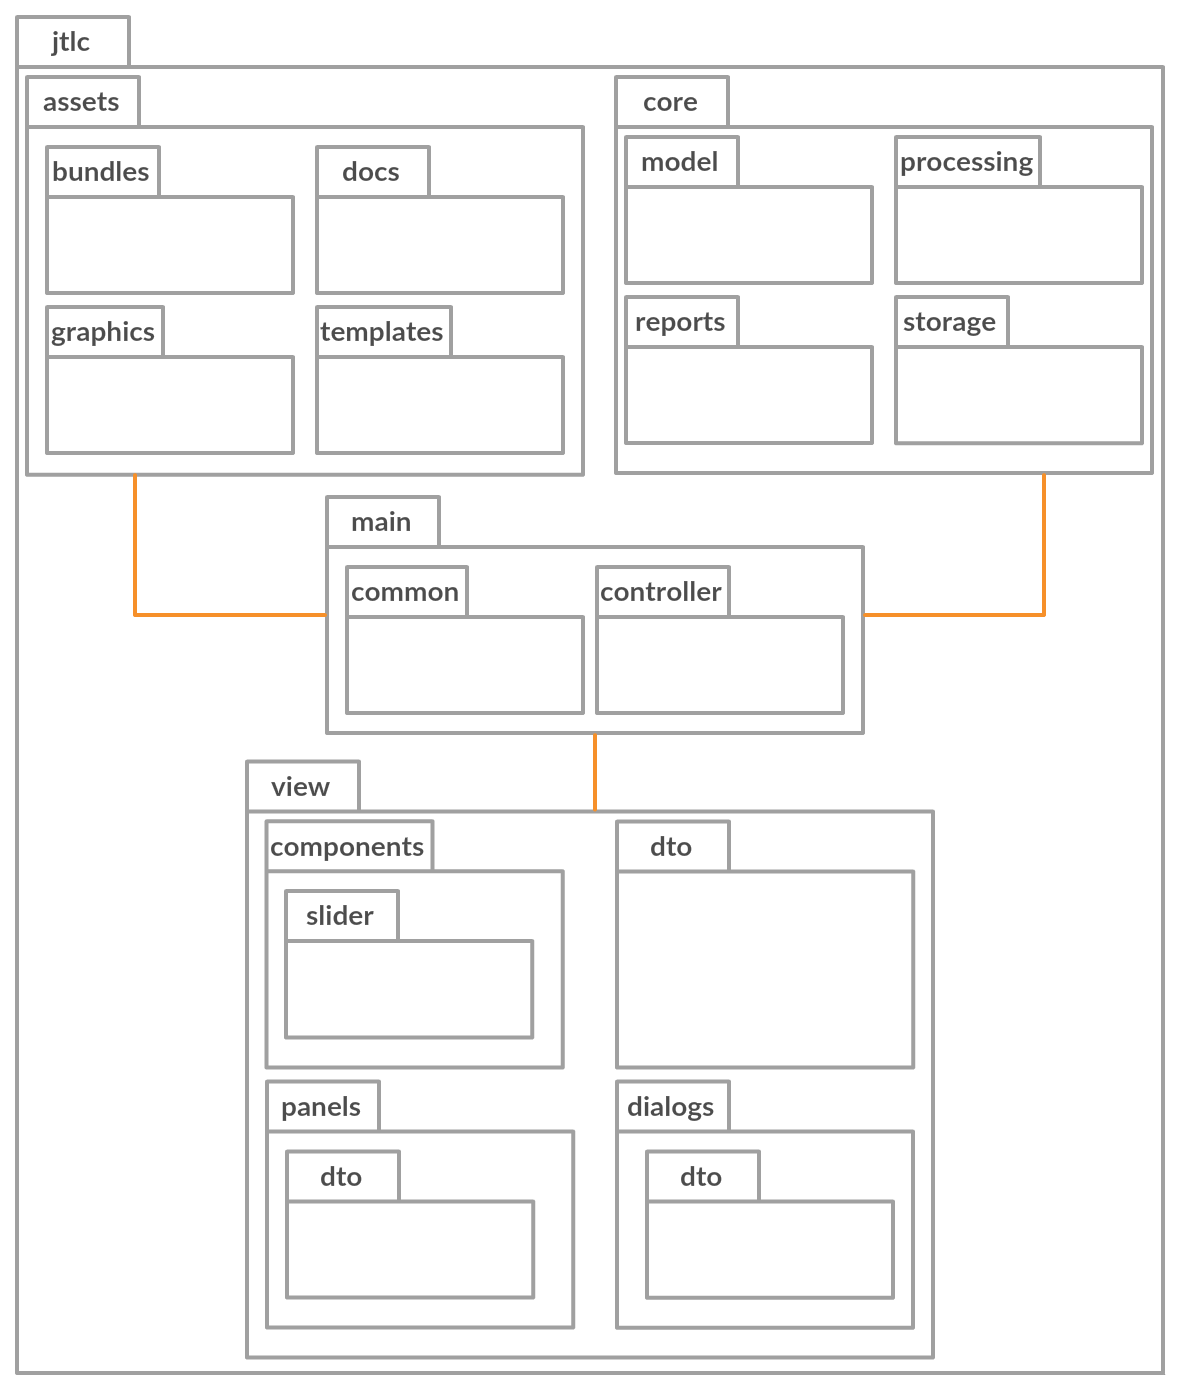
\includegraphics[width=400pt]{imagenes-jtlc/paquetes}
	\centering
	\vspace{-0.5cm}
	\caption{Diagrama de paquetes general del sistema.}
	\label{fig:disenoPaquetes}
\end{figure}

\section{Detalles de Implementaci\'on}
Como se detall\'o anteriormente, el sistema esta implementado en \textit{Java}, siguiendo la idea de dise\~no definida por el patr\'on arquitectural \textit{ MVC (Model-View-Controller)} destacando los 3 componentes principales Modelo, Vista y Controlador sumados a los componentes que permiten procesar las im\'agenes, realizar el an\'alisis de las muestras, la generaci\'on de informes, el almacenamiento de proyectos entre otros.

El n\'ucleo o \textit{core} (paquete \textit{jtlc.core}) del sistema esta compuesto por los paquetes \textit{Model, Processing, Reports} y \textit{Storage}.
Estos m\'odulos brindan las herramientas b\'asicas que permiten el an\'alisis de las muestras y la generaci\'on de reportes.\\
El modelo est\'a compuesto por 3 clases: \textit{Experiment, Sample} y \textit{Peak} pertenecientes al paquete \textit{jtlc.core.model} detallado en la figura \ref{fig:modeloDiagrama}. La clase \textit{Experiment} define la estructura b\'asica que posee un proyecto realizado en jTLC. Almacena los datos principales del proyecto, la imagen principal del experimento, la cual contiene las muestras a analizar; el par de puntos de cortes sobre la imagen principal, los cuales permiten recortar partes no deseadas de la imagen; el \'angulo de rotaci\'on de la imagen; los ejes de inversi\'on, que definen una combinaci\'on de ejes X - Y que permiten invertir vertical/horizontalmente la imagen; los comentarios, el titulo y la descripci\'on del proyecto, la fecha de creaci\'on y an\'alisis, entre otros. Es la estructura b\'asica del modelo, permite almacenar, obtener y actualizar los diferentes campos/atributos del experimento.
La clase \textit{Sample} implementa las estructuras de datos necesarias para almacenar la informaci\'on de una muestra en particular, como: los l\'imites de la muestra, la imagen recortada, el frente solvente, el punto de siembra, la media muestral, la superficie total de los picos, los comentarios y una lista de \textit{Peak}. \textit{Peak} define un pico de la media muestral de cada \textit{Sample}, almacena la posici\'on, el nombre, los l\'imites, la linea de base, la superficie (absoluta y relativa), el valor m\'aximo dentro del pico junto a su posici\'on y por \'ultimo la altura del mismo.

\begin{figure}[H]
	\centering
	\vspace{-0.5cm}
	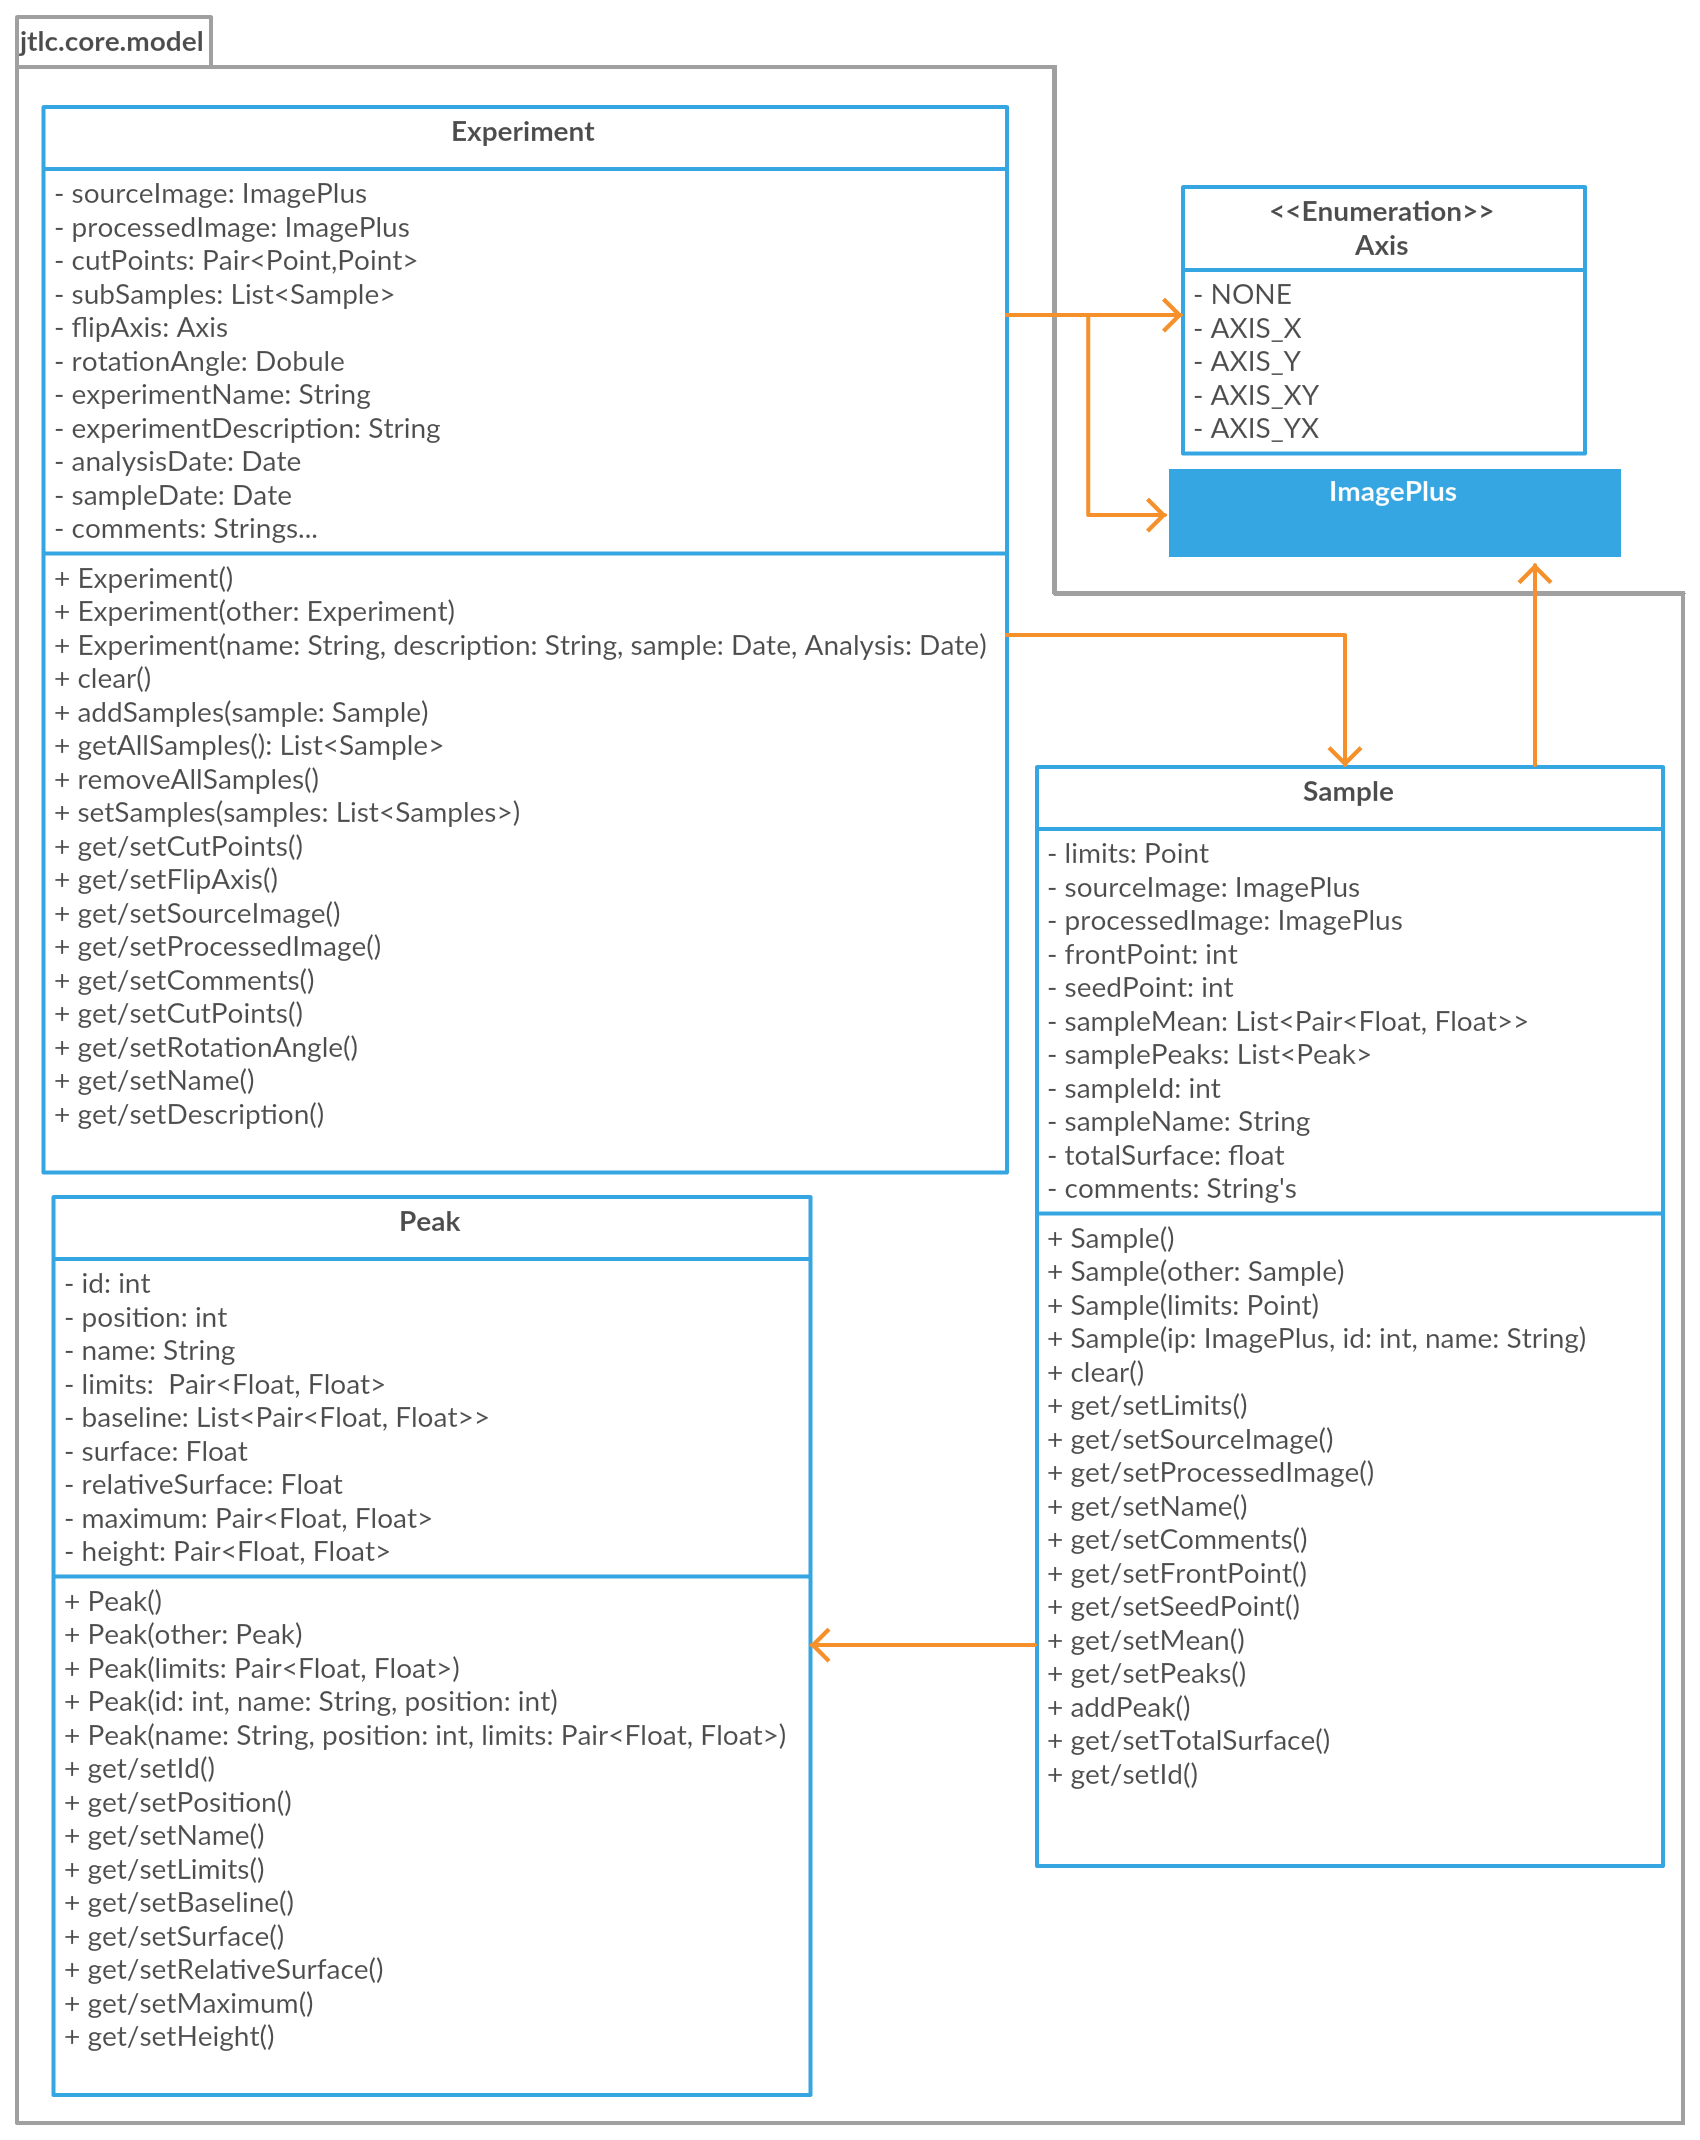
\includegraphics[width=425pt]{imagenes-jtlc/model}
	\centering
	\vspace{-0.5cm}
	\caption{Diagrama de Clases paquete \textit{jtlc.core.model}.}
	\label{fig:modeloDiagrama}
\end{figure}

El an\'alisis de las muestras se logra gracias a las funcionalidades brindadas por las clases \textit{ImageProcessing} y \textit{AnalisisProcessing}, pertenecientes al paquete \textit{jtlc.core.processing} el cual se detalla en la figura \ref{fig:processingDiagrama}. La clase \textit{ImageProcessing} brinda m\'etodos que permiten manipular f\'acilmente las im\'agenes cargadas, se basa en la libr\'ia \textit{ImageJ} \cite{imagej} para operar de manera unificada los diferentes formatos de im\'agenes, aplicar filtros, realizar operaciones y modificaciones, leer la matriz de p\'ixeles, entre otros. \textit{AnalisisProcessing} \'utiliza las funcionalidades provistas por la clase anterior para llevar a cabo el procesamiento de las im\'agenes que contienen las muestras a analizar. Facilita la b\'usqueda de los puntos de cortes, los l\'imites de cada muestra individual, permite computar la media muestral, buscar picos, buscar la linea de base de cada pico, validar \'areas de integraci\'on, integrar los picos, calcular los m\'aximos locales, la altura del pico, entre otros.

\begin{figure}[H]
	\centering
	\vspace{-0.5cm}
	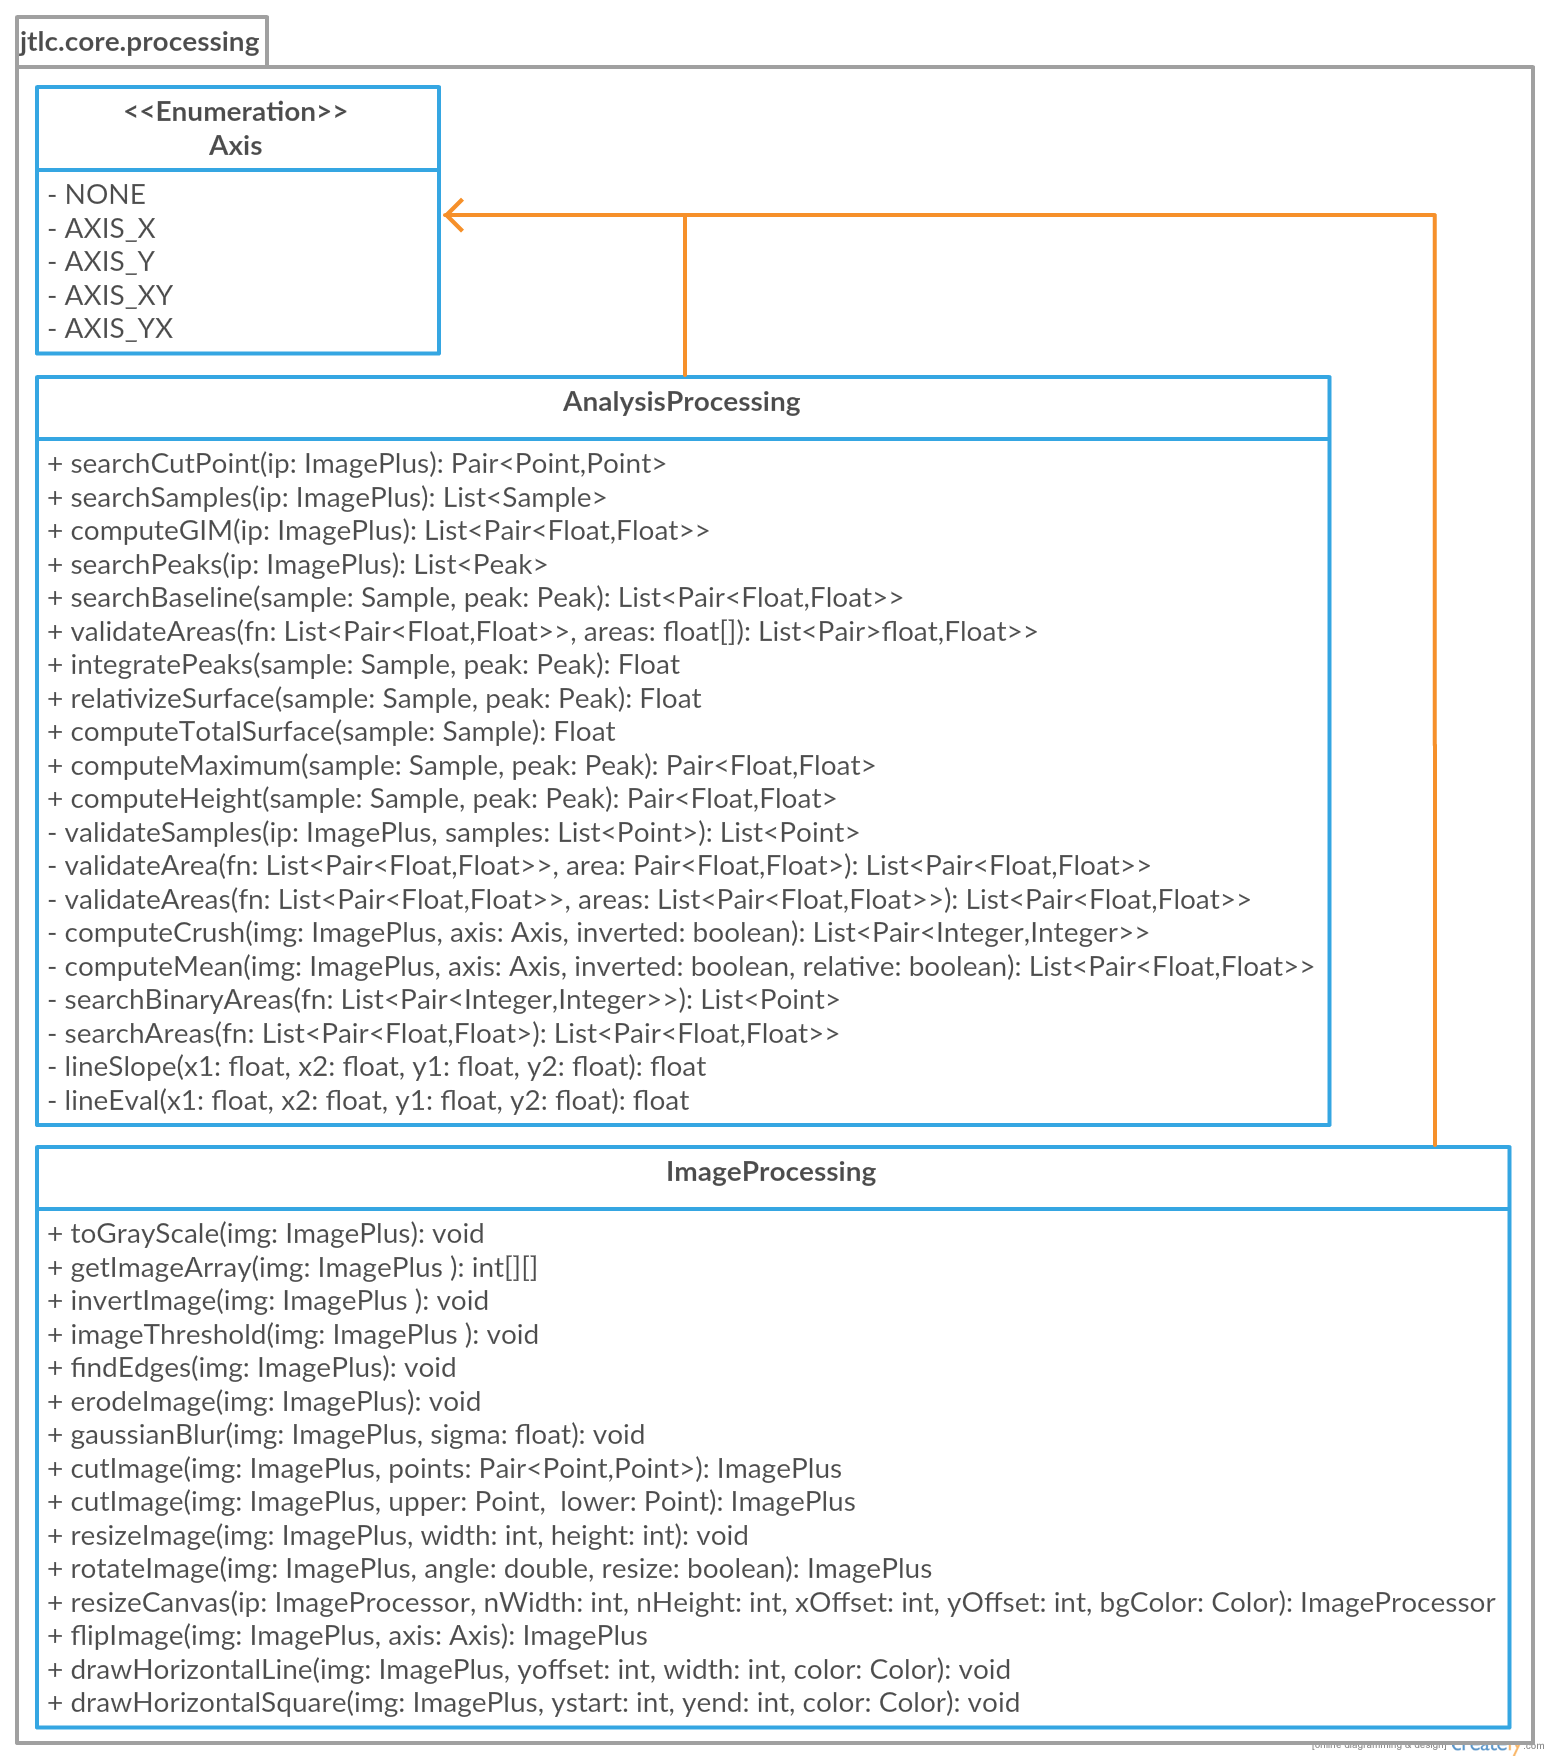
\includegraphics[width=425pt]{imagenes-jtlc/processing}
	\centering
	\vspace{-0.5cm}
	\caption{Diagrama de Clases paquete \textit{jtlc.core.processing}.}
	\label{fig:processingDiagrama}
\end{figure}

\newpage
Para la generaci\'on de reportes se \'utilizan las clases \textit{Reporter} y \textit{Template} pertenecientes al paquete \textit{jtlc.core.reports} (figura \ref{fig:reportsDiagrama}). \textit{Reporter} se encarga de generar la estructura b\'asica de un reporte, se basa en un \textit{Template} sobre el cual va llenando los diferentes campos con los resultados del proceso de an\'alisis.
\'Utiliza un template en formato ODT el cual es f\'acilmente accedido gracias a la clase \textit{Template}, permite generar reportes en diferentes idiomas, seg\'un el idioma actual de la aplicaci\'on, as\'i como tambi\'en, permite exportar los reportes en formatos ODT, PDF, HTML, CSV y TXT.

\begin{figure}[H]
	\centering
	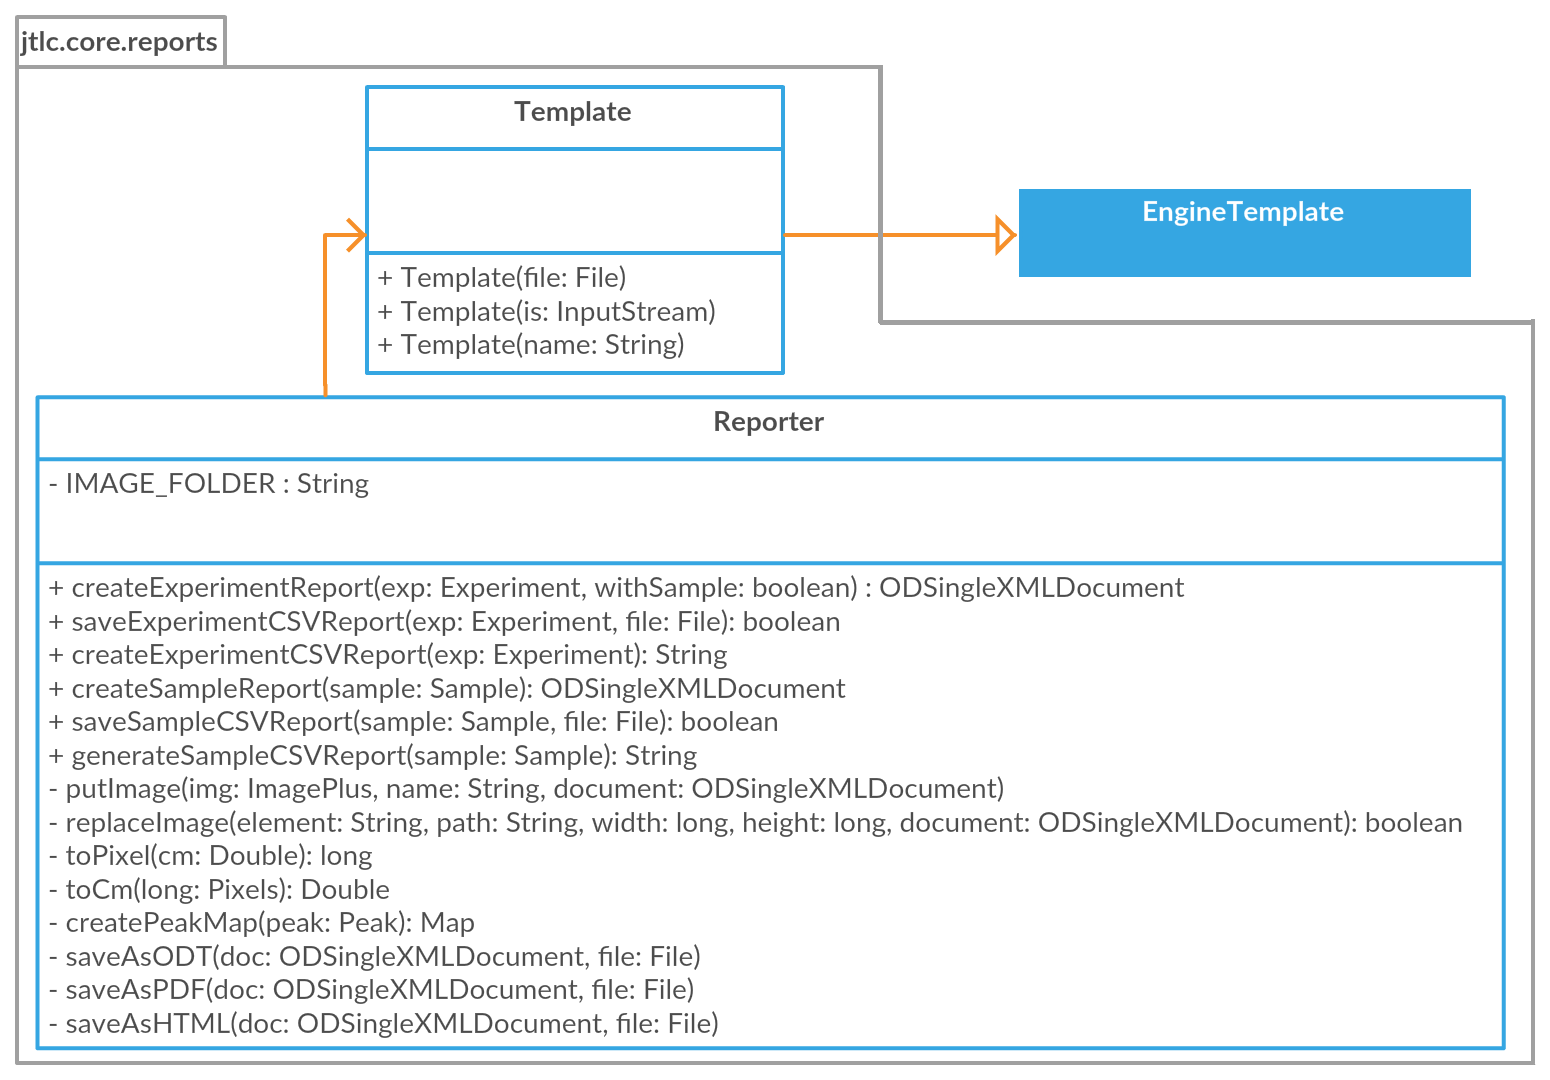
\includegraphics[width=425pt]{imagenes-jtlc/reports}
	\centering
	\vspace{-0.5cm}
	\caption{Diagrama de Clases paquete \textit{jtlc.core.reports}.}
	\label{fig:reportsDiagrama}
\end{figure}

El almacenamiento de los proyectos se logra gracias a las clases pertenecientes al paquete \textit{jtlc.core.storage} (figura \ref{fig:storageDiagrama}). El paquete esta compuesto por las clases \textit{ImageStore}, \textit{ModelSaver}, \textit{ModelLoader}. La clase \textit{ImageStore} brinda m\'etodos que permiten f\'acilmente cargar im\'agenes desde el sistema de archivos, as\'i como tambi\'en permite almacenarlas en diferentes formatos, ya sea en disco o en memoria para luego ser procesadas nuevamente. La clase \textit{ModelSaver} permite guardar los datos del experimento actual en diferentes formatos, brinda la posibilidad de guardar datos en archivos de texto o almacenar todo el proyecto en un formato comprimido (\textit{ZIP}), el cual incluye un archivo \textit{XML} con los datos y resultados del experimento, las distintas im\'agenes procesadas y generadas durante el an\'alisis as\'i como la media muestral de cada muestra individual en el experimento. La clase \textit{ModelLoader} brinda funcionalidades que permiten cargar en el sistema experimentos previamente guardados usando el m\'odulo anterior, permite tambi\'en leer una lista de proyectos dentro de una carpeta del sistema, cargando todos los proyectos que all\'i se encuentren. El proceso de carga inicia por leer el archivo comprimido (formato \textit{ZIP} con extensi\'on .jtlc), primero lee el archivo \textit{XML} donde se almacenan todos los datos del proyecto y donde se encuentran las rutas relativas a las im\'agenes del proyecto a cargar, generando as\'i un experimento que puede ser nuevamente cargado en el sistema para continuar su procesado o revisar los resultados previamente obtenidos.

\begin{figure}[H]
	\centering
	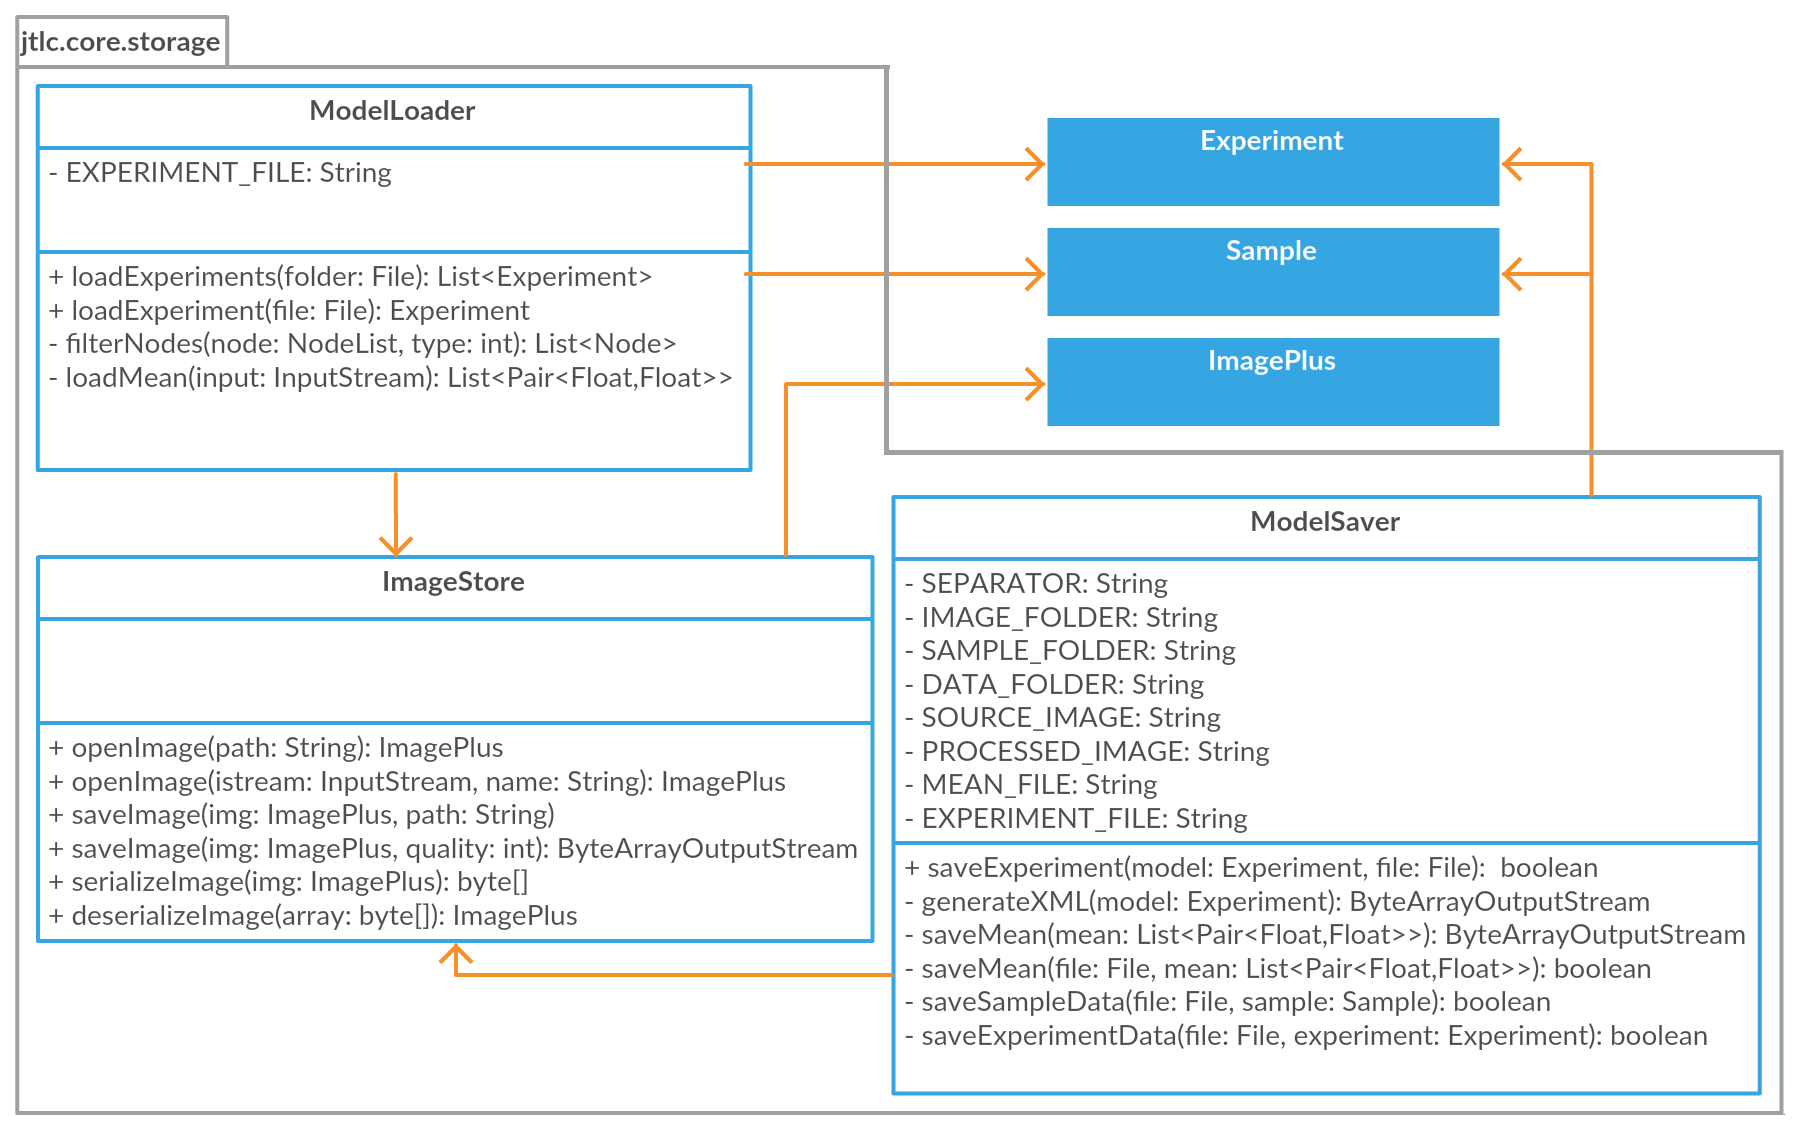
\includegraphics[width=425pt]{imagenes-jtlc/storage}
	\centering
	\vspace{-0.5cm}
	\caption{Diagrama de Clases paquete \textit{jtlc.core.storage}.}
	\label{fig:storageDiagrama}
\end{figure}

\newpage
El paquete \textit{jtlc.assets} agrupa los recursos del sistema, contiene los elementos gr\'aficos o \'iconos, los \textit{templates} (plantillas) para la generaci\'on de reportes, los documentos de ayudas, las licencias as\'i como los recursos de idiomas. Concentra toda su funcionalidad de la clase principal \textit{Assets} la cual permite cargar f\'acilmente la iconograf\'ia del sistema, los textos de cada elemento seg\'un el idioma seleccionado, implementa la actualizaci\'on de los textos durante el cambio de idiomas, permite cargar los \textit{templates} para generar los reportes, cargar los documentos de informaci\'on, entre otros. En la figura \ref{fig:assetsDiagrama} se detalla el contenido general del paquete, con \'enfasis sobre la clase \textit{Assets}

\begin{figure}[H]
	\centering
	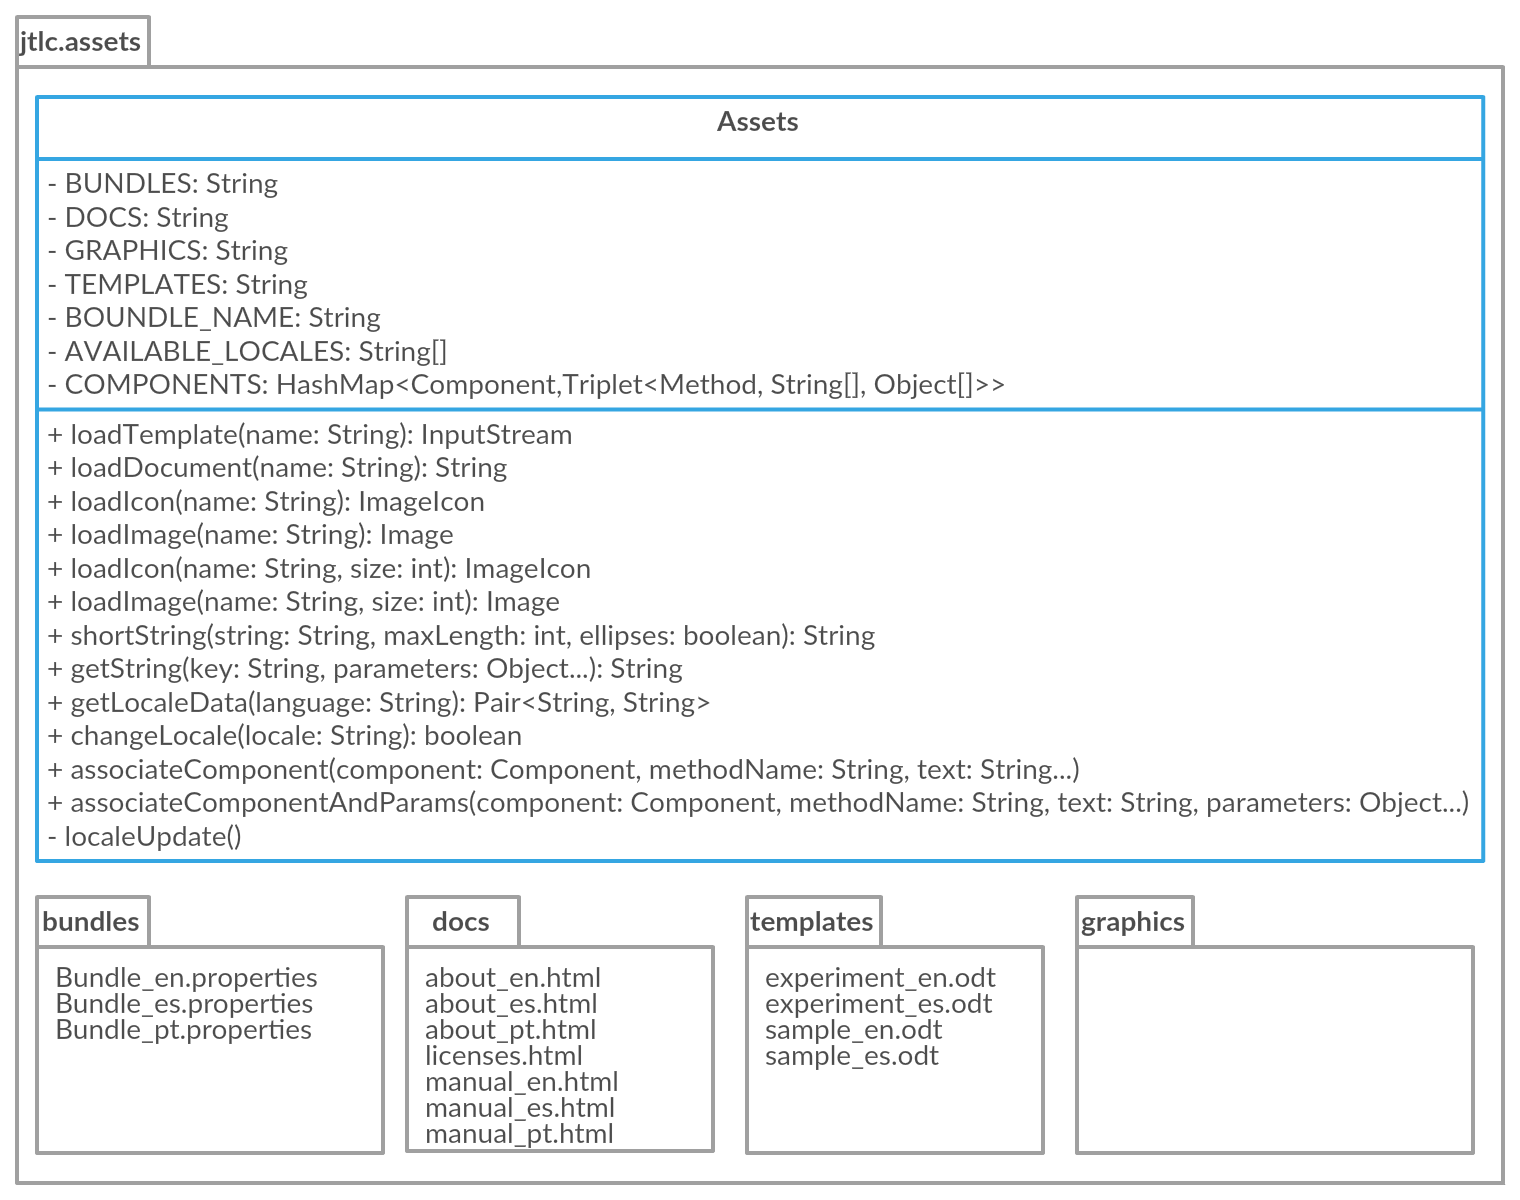
\includegraphics[width=425pt]{imagenes-jtlc/assets}
	\centering
	\vspace{-0.5cm}
	\caption{Diagrama de Clases paquete \textit{jtlc.assets}.}
	\label{fig:assetsDiagrama}
\end{figure}

\newpage
La interfaz gr\'afica esta formada por las clases contenidas en el paquete \textit{jtlc.view} (figura \ref{fig:viewDiagrama}), el cual agrupa todos los componentes que forman las diferentes ventanas y paneles que permiten interactuar con el sistema. La vista principal de la aplicaci\'on esta implementada en la clase \textit{MainView}, la cual \'utiliza los elementos provistos por los subpaquetes dentro de \textit{jtlc.view} extendiendo de la clase \textit{Observable} lo que le permite f\'acilmente comunicar los cambios ocurridos al controlador (\textit{Observer}) por medio de notificaciones simples. El subpaquete \textit{dto} define las estructuras b\'asicas que permiten compartir informaci\'on entre las vistas y los controladores (\textit{DTO (Data Transfer Object)}), define la clase abstracta \textit{AbstractDTO} la cual brinda una estructura com\'un a todos los \textit{DTO's} del sistema y permite marcar f\'acilmente si hubieron cambios durante el proceso de una vista o panel.
El subpaquete \textit{dialogs} contiene los diferentes cuadros de d\'ialogos \'utilizados en el sistema, como as\'i tambi\'en los \textit{DTO's} necesarios para comunicar los datos entre los d\'ialogos y el controlador. Define una interfaz \textit{IDialog} com\'un a todos los cuadros de d\'ialogo que permite obtener los resultados de manera simple y transparente. En la figura \ref{fig:dialogsDiagrama} se resume el paquete de forma general. Las diferentes ventanas o di\'alogos son:
\begin{itemize}
	\item \textit{ProjectDialog}: Este di\'alogo se \'utiliza al momento de crear un nuevo proyecto, permite introducir los datos b\'asicos del experimento. Da como resultado un \textit{ProjectDTO} conteniendo los datos ingresados.
	\item \textit{SettingsDialog}: Permite visualizar y establecer las configuraciones del sistema. Toma como entrada un \textit{SettingsDTO} con la configuraci\'on actual y da como resultado un objeto del mismo tipo contiendo la nueva configuraci\'on en el caso que se registren cambios en la misma.
	\item \textit{InfoDialog}: Muestra la informaci\'on del proyecto actual, permite cambiar los datos (editar) del mismo. Su entrada es un \textit{InfoDTO} con los datos actuales del proyecto y su resultado es un objeto del mismo tipo con los nuevos datos en el caso que se realice alg\'un cambio.
	\item \textit{ImageExportDialog}: Permite exportar im\'agenes del experimento al sistema de archivos, as\'i como tambi\'en redimensionar la imagen al momento del guardado. Su entrada es un objeto \textit{ImageExportDTO} conteniendo informaci\'on sobre la imagen a exportar (tama\~no, vista previa, etc) y su resultado es un objeto del mismo tipo conteniendo el tama\~no de exportaci\'on deseado.
	\item \textit{TextPanelDialog}: Este cuadro de di\'alogo se encarga de mostrar un \'area de texto plano o en formato \textit{HTML}. Su entradas son: el texto a mostrar, el t\'itulo de la ventana y el \'icono de la misma. No da como resultado ning\'un valor.
\end{itemize}

\begin{figure}[H]
	\centering
	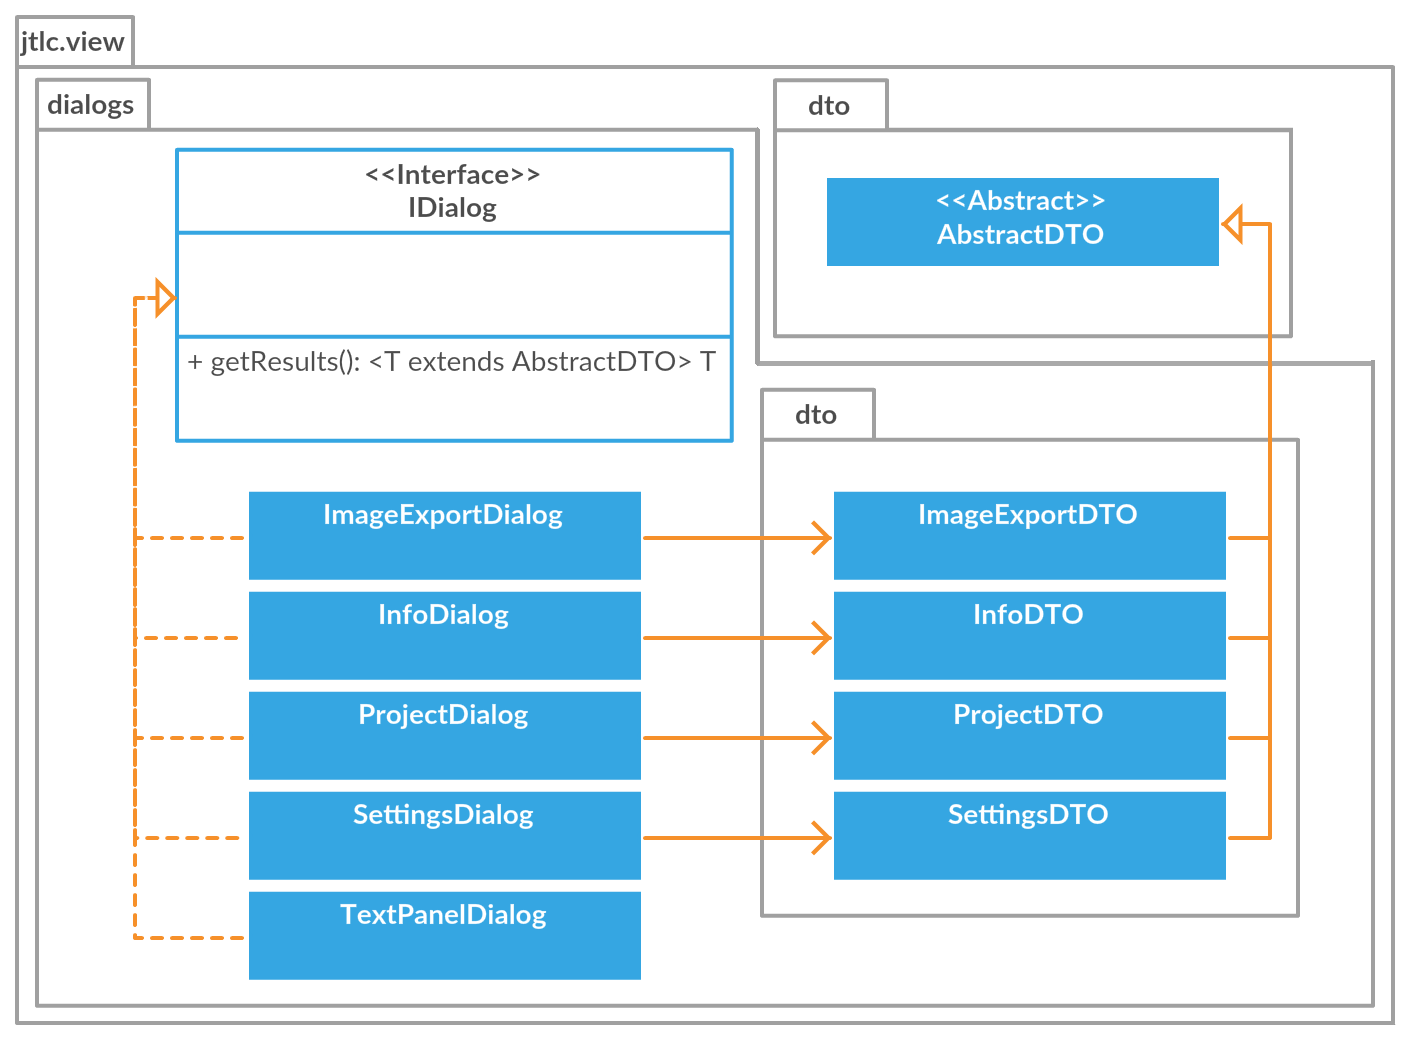
\includegraphics[width=425pt]{imagenes-jtlc/dialogs}
	\centering
	\vspace{-0.5cm}
	\caption{Diagrama de Clases paquete \textit{jtlc.view.dialogs}.}
	\label{fig:dialogsDiagrama}
\end{figure}

\begin{figure}[H]
	\centering
	\vspace{-2.5cm}
	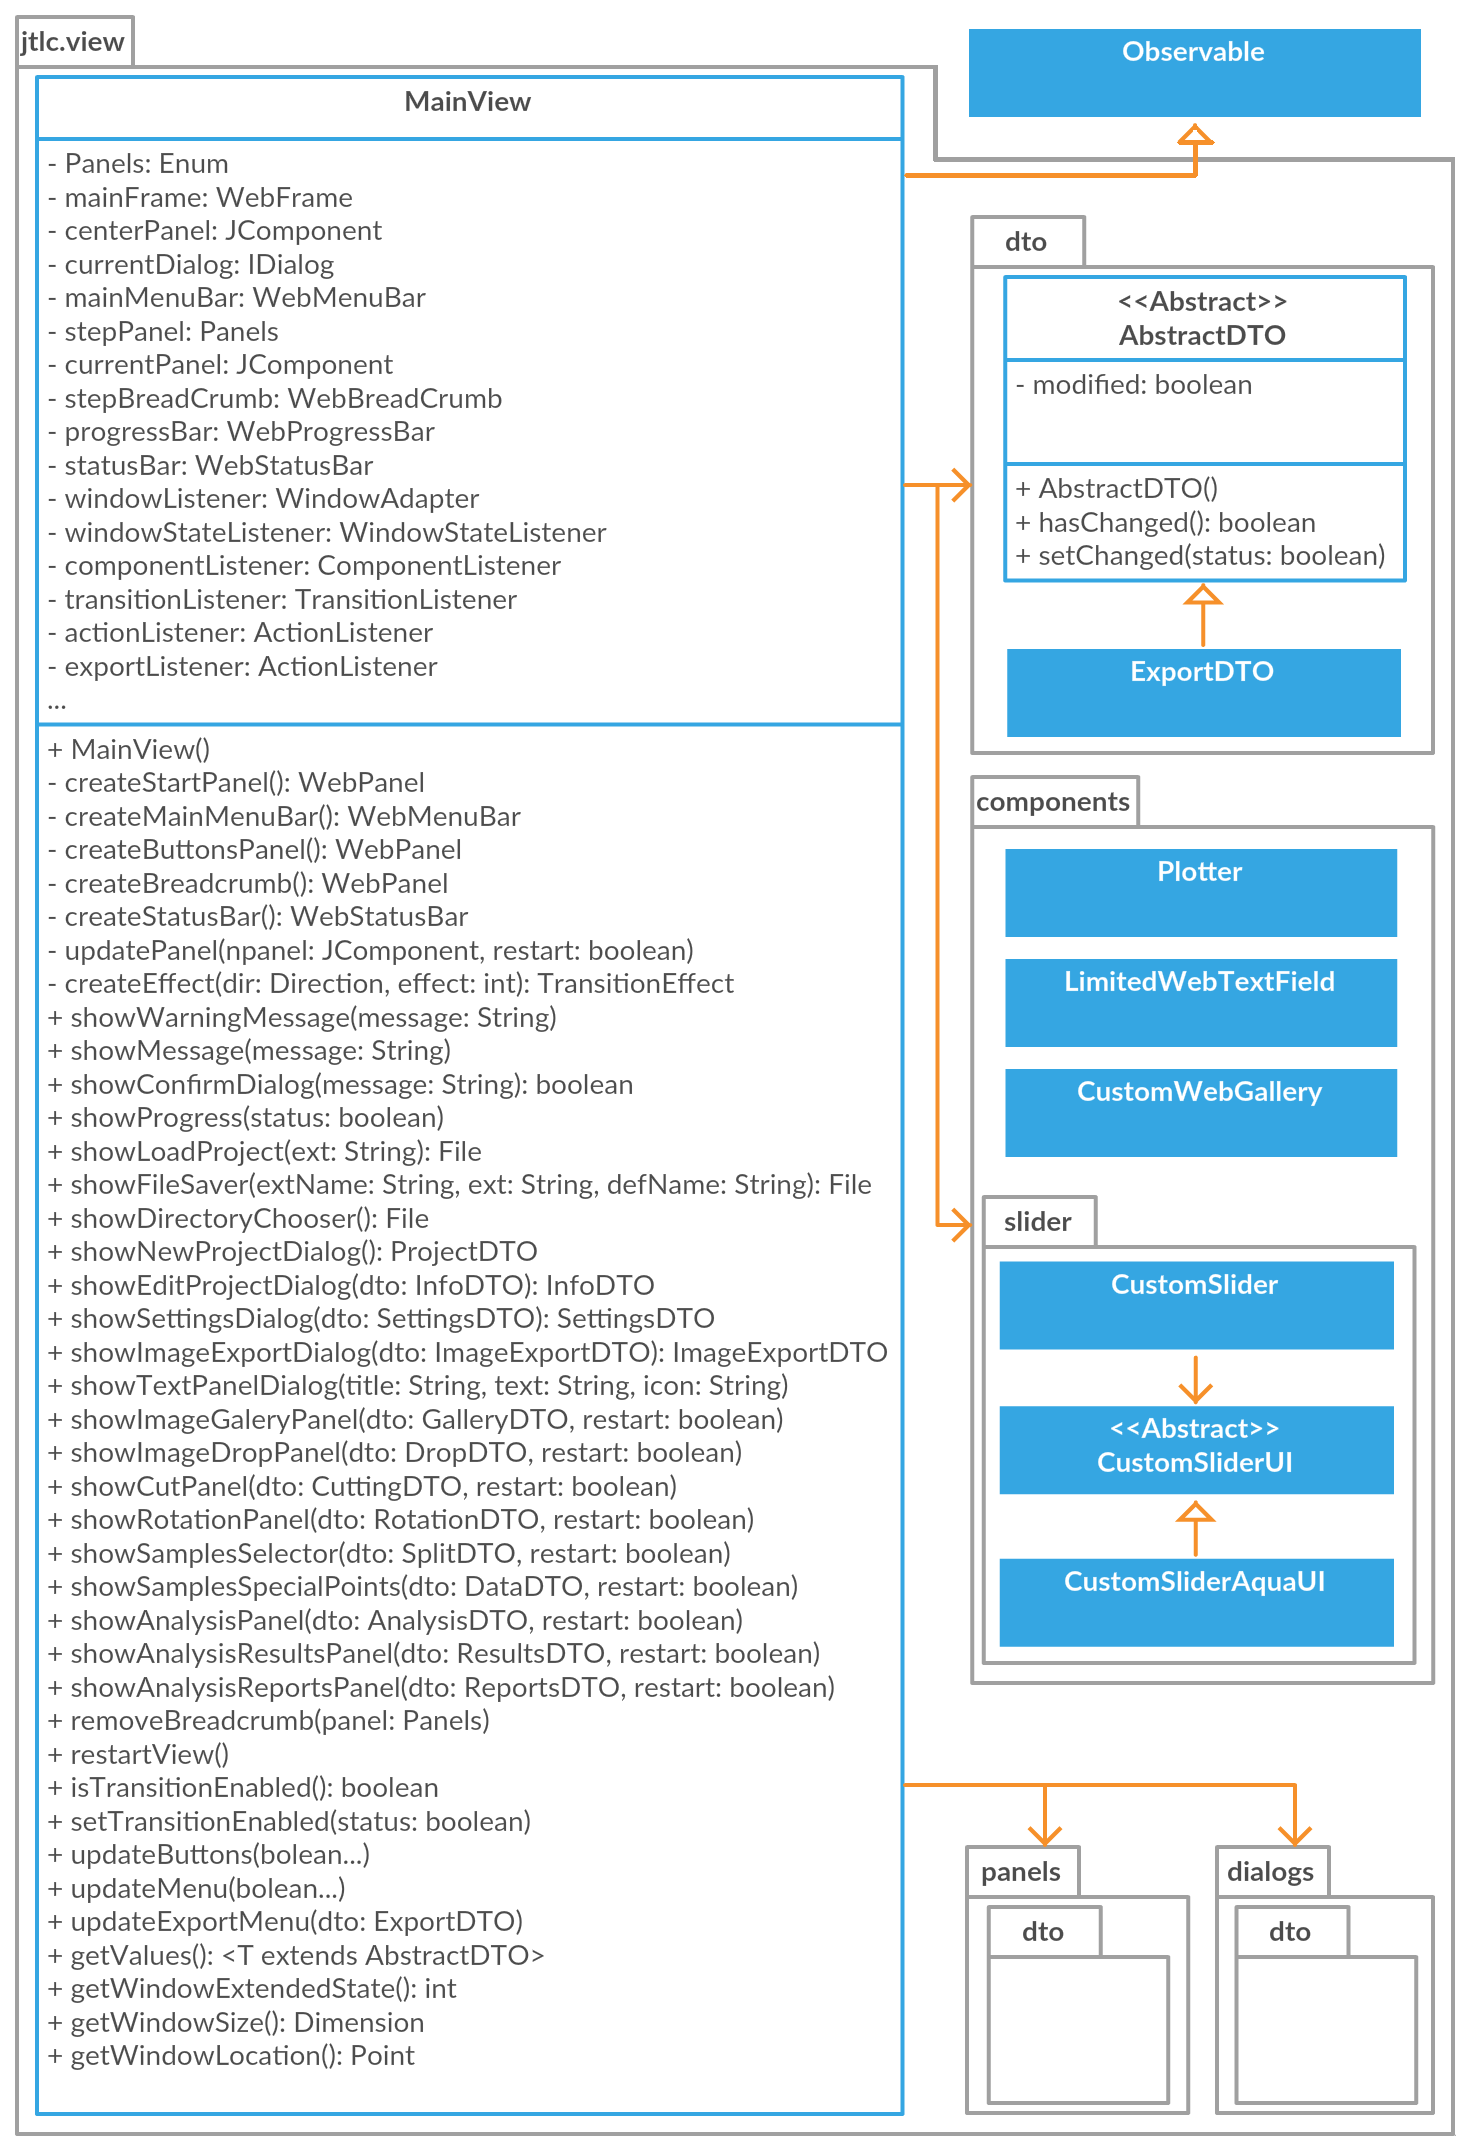
\includegraphics[width=425pt]{imagenes-jtlc/view}
	\centering
	\vspace{-1.0cm}
	\caption{Diagrama de Clases paquete \textit{jtlc.view}.}
	\label{fig:viewDiagrama}
\end{figure}

El subpaquete \textit{panels} contiene los paneles principales del sistema que se \'utilizan durante el an\'alisis de las muestras. Define una interfaz com\'un a todos los paneles que f\'acilita la interacci\'on con los controladores. Dentro se define el subpaquete \textit{dto} el cual contiene todos los \textit{dto's} que permiten la interacci\'on con los diferentes paneles, los cuales se basan en la clase \textit{AbstractDTO} para generalizar y facilitar su uso. En la figura \ref{fig:panelsDiagrama} se resume el paquete en forma general. Los diferentes paneles son:
\begin{itemize}
	\item \textit{GalleryPanel}: Es el encargado de mostrar la galer\'ia de proyectos al momento de explorar un directorio. \'Utiliza la clase \textit{CustomWebGallery} en su implementaci\'on y as\'i permitir elegir un proyecto para continuar a trav\'es de una galer\'ia de im\'agenes. Su entrada es un \textit{GalleryDTO} conteniendo la lista de posibles experimentos a cargar y su resultado es el mismo objeto conteniendo la informaci\'on sobre el proyecto elegido.
	\item \textit{DropPanel}: Este panel permite cargar la imagen inicial del proyecto, es el primer panel visible durante el proceso del experimento. Implementa un \'area \textit{Drag \& Drop} que facilita la carga de im\'agenes con un simple arrastrar y soltar, tambi\'en permite explorar el sistema de archivos buscando manualmente la imagen deseada a trav\'es de un selector de archivos est\'andar. Su entrada es un \textit{DropDTO} conteniendo la imagen inicial a mostrar y los comentarios previamente guardados, su resultado es un objeto del mismo tipo conteniendo la imagen cargada y los nuevos comentarios ingresados.
	\item \textit{CutPanel}: Permite recotar \'areas de la imagen del experimento. Muestra la imagen de fondo y dos gu\'ias (una horizontal y otra vertical) que definen un recuadro sobre la misma delimitando el \'area final de la imagen recortada. Su entrada es un \textit{CuttingDTO} conteniendo la imagen a procesar y un par de puntos que definen el \'area previamente establecida por el asistente de procesado. Su resultado es un objeto del mismo tipo conteniendo la nueva \'area seleccionada en caso de que haya ocurrido alg\'un cambio, ademas posee informaci\'on sobre los comentarios realizados en este proceso.
	\item \textit{RotationPanel}: El panel de rotaci\'on permite realizar transformaciones b\'asicas sobre la imagen del experimento. Brinda la posibilidad de rotar la imagen de manera arbitraria cualquier cantidad de grados, invertir la imagen tanto sea horizontal como verticalmente o realizar rotaciones a escuadra. Su entrada es un \textit{RotationDTO} conteniendo la imagen a procesar, los datos de rotaci\'on e inversi\'on previamente establecidos, su resultado es un objeto del mismo tipo conteniendo las nuevas transformaciones aplicadas de haber ocurrido junto a los comentarios realizados en esta etapa del proceso.
	\item \textit{SplitPanel}: Es el encargado de separar las muestras en im\'agenes individuales. Permite seleccionar manualmente a trav\'es de lineas de gu\'ia los puntos donde empieza y termina cada muestra a analizar. Su entrada es un \textit{SplitDTO} conteniendo la imagen a procesar y los puntos de separaci\'on previamente calculados por el asistente de proceso, su resultado es un objeto del mismo tipo conteniendo los nuevos puntos de separaci\'on en el caso que el usuario haya realizado alg\'un cambio junto a los comentarios realizados en este proceso.
	\item \textit{DataPanel}: Este panel permite ingresar los datos espec\'ificos de cada muestra individual. Permite seleccionar el punto de siembra y el frente solvente de cada una, de manera global, es decir, el mismo para todas las muestras, o de manera individual. A su vez permite establecer el nombre de la muestra, comentarios individuales para cada una de ellas o comentarios globales a toda la etapa del proceso. Su entrada es un \textit{DataDTO} conteniendo las im\'agenes de cada muestra individual, y los datos previamente cargados de cada una de ellas. Su resultado es un objeto del mismo tipo conteniendo los nuevos datos cargados de ser necesario.
	\item \textit{AnalysisPanel}: En el panel de an\'alisis se realiza el an\'alisis de cada muestra a partir del gr\'afico de la media muestral obtenida durante el proceso. Permite seleccionar los picos individuales mediante un \textit{Slider} sobre el gr\'afico o sobre la imagen fuente. Tambi\'en permite visualizar la comparaci\'on de la media de cada muestra y realizar comentarios individuales a cada una de ellas. La entrada de este panel es un \textit{AnalysisDTO} conteniendo la media de cada muestra, los l\'imites de cada pico calculados por el asistente de proceso, los comentarios previamente realizados y los datos de cada muestra. Su resultado es un objeto del mismo tipo conteniendo los nuevos comentarios y los nuevos l\'imites de cada pico.
	\item \textit{ResultsPanel}: En este panel se muestran los resultados obtenidos durante el proceso de an\'alisis junto a los datos de cada muestra. Se detallan los datos de cada pico, su superficie total y relativa, los l\'imites, la altura, el valor m\'aximo, la l\'inea de base, entre otros. Su entrada es un \textit{ResultsDTO} conteniendo los resultados de cada muestra y sus datos, su salida es un objeto del mismo tipo conteniendo los comentarios realizados en esta etapa. Tambi\'en permite establecer el nombre a cada pico individualmente para cada muestra procesada.
	\item \textit{ReportsPanel}: El panel de Reportes muestra los reportes con los datos de las muestras y los resultados del an\'alisis as\'i como tambi\'en los datos del experimento. Su entrada es un \textit{ReportsDTO} conteniendo los datos a mostrar. No produce ning\'un resultado espec\'ifico.
\end{itemize}

\begin{figure}[H]
	\centering
	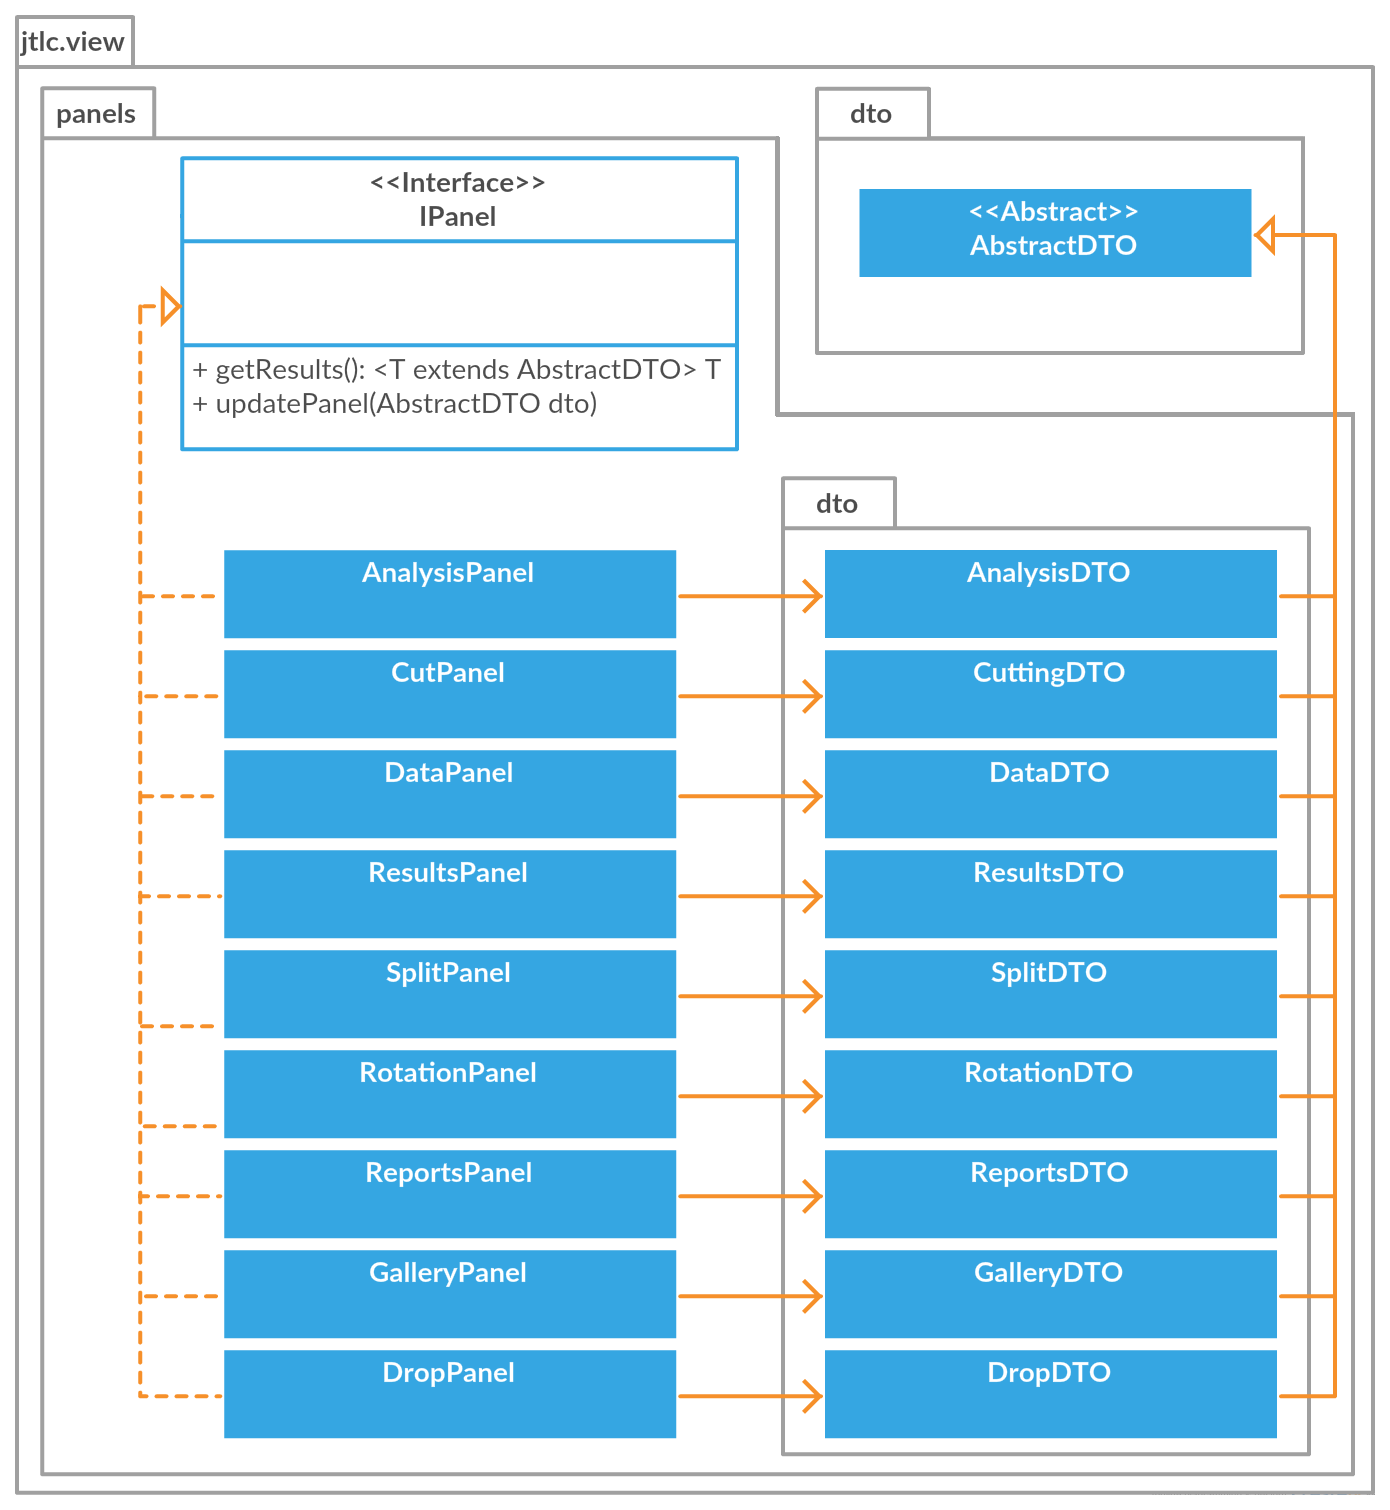
\includegraphics[width=425pt]{imagenes-jtlc/panels}
	\centering
	\vspace{-0.5cm}
	\caption{Diagrama de Clases paquete \textit{jtlc.view.panels}.}
	\label{fig:panelsDiagrama}
\end{figure}

\newpage
Por \'ultimo el paquete \textit{components} contiene los componentes personalizados del sistema que se utilizan a lo largo de diferentes paneles, principalmente los \textit{Sliders} que permiten delimitar \'areas y el \textit{Plotter} que se encargar de graficar la curva resultante de la media muestral de cada muestra analizada junto a la informaci\'on b\'asica de los picos, la l\'inea de base y el \'area de integraci\'on. Los \textit{Sliders} est\'an implementados por la clase \textit{CustomSlider} la cual se basa en la librer\'ia \textit{MultiThumbSlider} parte del paquete \textit{JavaGraphics (https://javagraphics.java.net/)} provista por \textit{Jeremy Wood} agregando detalles personalizados que brindan funcionalidad extra como las l\'ineas de gu\'ia, emparejar dos \textit{thumbs}, dibujar el \'area de selecci\'on o recuadro entre dos \textit{thumbs}, etc. El \textit{Plotter} desarrolla un \textit{JComponent} personalizado el cual a partir de gr\'aficos 2D se encarga de dibujar o realizar un plot de un conjunto de valores en X e Y. En esta aplicaci\'on se \'utiliza para dibujar la media muestral de cada muestra junto al \'area de integraci\'on de cada pico, su l\'inea de base y otros datos relacionados. En la figura \ref{fig:componentsDiagrama} se detalla la implementaci\'on del paquete.

\begin{figure}[H]
	\centering
	\vspace{-1.5cm}
	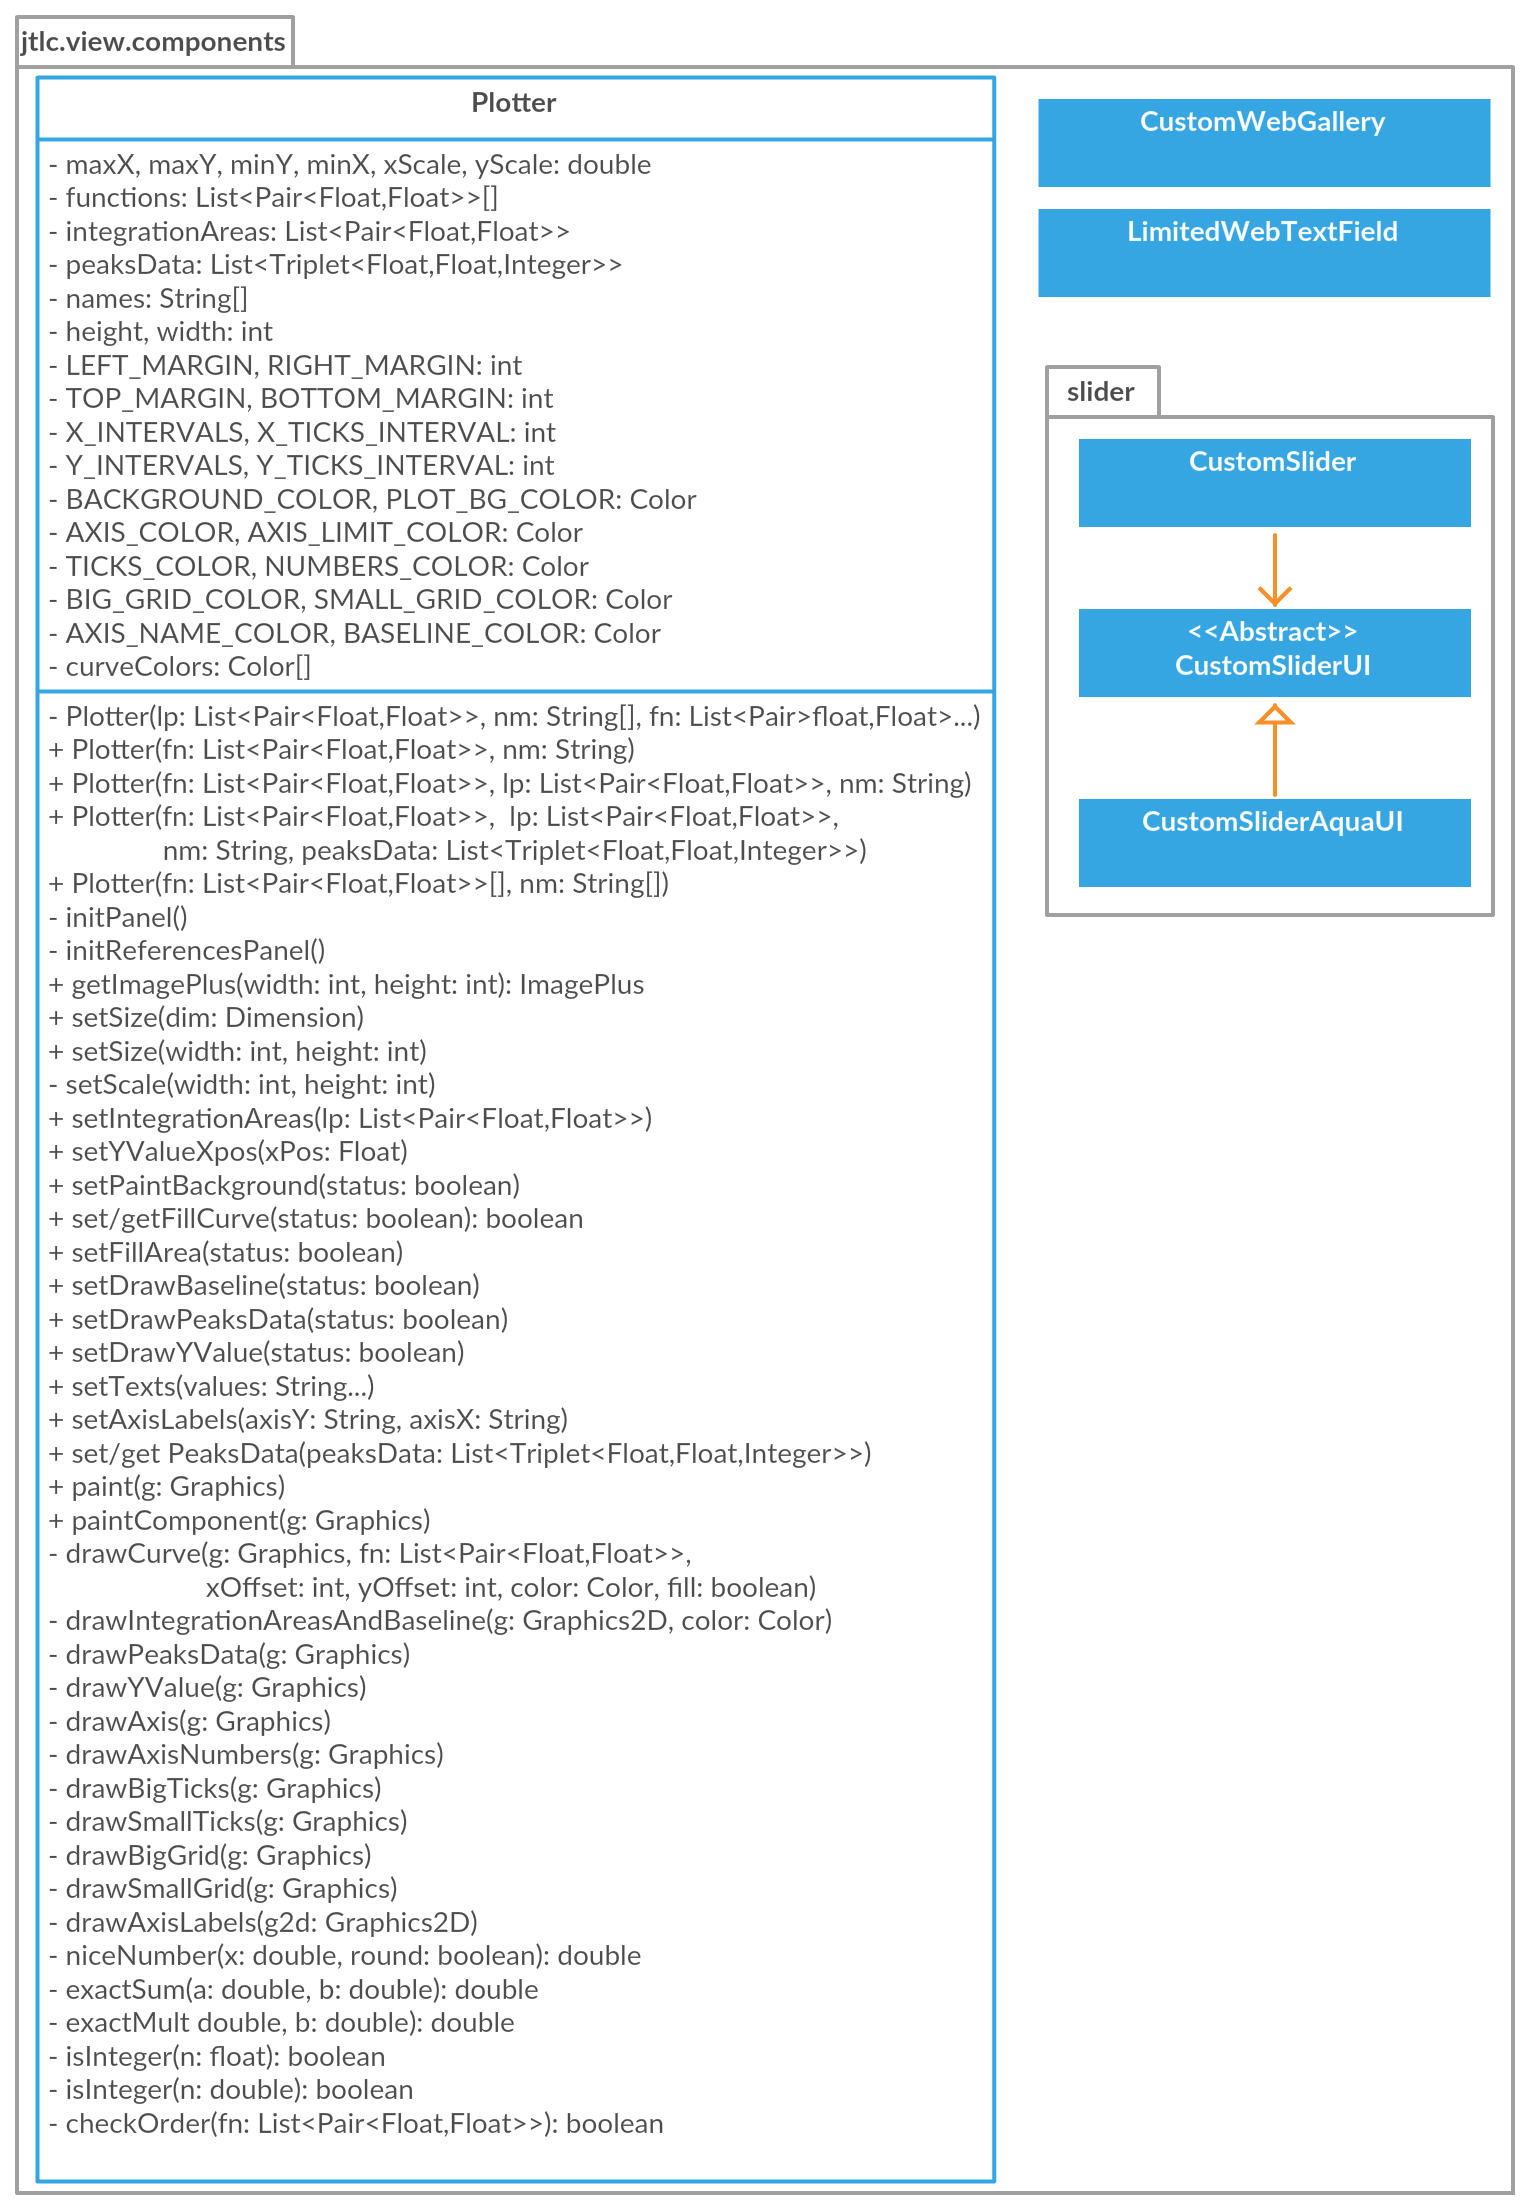
\includegraphics[width=425pt]{imagenes-jtlc/components}
	\centering
	\vspace{-0.5cm}
	\caption{Diagrama de Clases paquete \textit{jtlc.view.panels}.}
	\label{fig:componentsDiagrama}
\end{figure}

El paquete \textit{jtlc.main} (figura \ref{fig:mainDiagrama}) contiene los principales componentes que permiten inicializar y controlar la ejecuci\'on de la aplicaci\'on, se subdivide en tres paquetes \textit{main}, \textit{common} y \textit{controller}. El primero contiene la clase principal que se encarga de la ejecuci\'on del sistema, inicializar las vistas y crear el controlador principal de la aplicaci\'on. El subpaquete \textit{common} contiene las estructuras b\'asicas que son \'utilizadas a lo largo de todo el sistema, la clase \textit{Point} que implementa un par de \textit{Integers}, la clase \textit{Pair} que implementa un par gen\'erico de dos elementos, la clase \textit{Triplet} la cual extiende \textit{Pair} agregando un elemento mas al conjunto y por \'ultimo la clase \textit{Settings} que permite guardar y cargar la configuraci\'on previa del sistema o crear la configuraci\'on por defecto en el caso que sea la primera ejecuci\'on, usando un patr\'on \textit{Singleton} para su cometido. El subpaquete \textit{controller} (figura \ref{fig:controllerDiagrama}) contiene las clases que implementan el control de la aplicaci\'on: \textit{Action} y \textit{Controller}. La primera define una Anotaci\'on \textit{Java} que permite identificar una acci\'on a ejecutar dentro del controlador a trav\'es de un \textit{String} de comando. El \textit{Controller} se encarga de controlar el progreso de la aplicaci\'on durante el proceso de an\'alisis as\'i como tambi\'en manejar la acciones de los diferentes cuadros de d\'ialogo. Implementa un \textit{Observer} el cual esta escuchando a los cambios o notificaciones producidas por las vistas. Define un m\'etodo \textit{update} el cual es ejecutado cuando ocurre un cambio o en respuesta a una determinada acci\'on. Este m\'etodo se encarga de derivar la responsabilidad de la respuesta a los diferentes servicios brindados por la clase a trav\'es de las anotaciones definidas en cada uno de ellos, busca entre todos los m\'etodos definidos en la clase cual es el que corresponde ejecutar al comando requerido seg\'un la acci\'on definida por la anotaci\'on \textit{Action} del m\'etodo. Para mejorar en eficiencia, al momento de inicializar el controlador, se crea tambi\'en un \textit{HashMap} conteniendo la acci\'on definida por la anotaci\'on del m\'etodo como clave y una referencia al mismo m\'etodo como valor, de esta forma al momento de responder a una determinada acci\'on solo se debe obtener a partir del mapa cual es el m\'etodo que corresponde a dicha acci\'on. Las acciones definidas por el controlador son:
\begin{itemize}
	\item \textit{NEW\_PROJECT}: Ejecuta el m\'etodo \textit{newProject} el cual muestra el cuadro de di\'alogo para crear un nuevo proyecto, inicializa las estructuras del nuevo proyecto con los datos ingresados, muestra el primer paso del proceso.
	\item \textit{LOAD\_PROJECT}: Ejecuta el m\'etodo \textit{loadProject} el cual muestra el cuadro de di\'alogo para cargar un proyecto previamente guardado, continua cargando el proyecto seleccionado mostrando el primer paso del proceso.
	\item \textit{EXPLORE\_PROJECTS}: Ejecuta el m\'etodo \textit{exploreProjects} mostrando el cuadro de di\'alogo de selecci\'on de directorio, muestra la galer\'ia de proyectos contenidos en el directorio.
	\item \textit{SAVE\_AS\_PROJECT}: Ejecuta el m\'etodo \textit{saveProject}, muestra el cuadro de di\'alogo para seleccionar o crear un archivo, escribe los datos del experimento actual al archivo seleccionado usando los servicios brindados por \textit{ModelSaver}.
	\item \textit{SAVE\_PROJECT}: Ejecuta el m\'etodo \textit{overwriteProject}, disponible en el caso que exista un archivo previo del proyecto actual. Sobrescribe el archivo con los nuevos datos del proyecto.
	\item \textit{EXIT\_SYSTEM}: Ejecuta el m\'etodo \textit{exitSystem}, el cual finaliza la instancia actual de la aplicaci\'on.
	\item \textit{EDIT\_PROJECT}: Ejecuta el m\'etodo \textit{editProyect} el cual muestra el cuadro de di\'alogo que permite editar los datos b\'asicos del proyecto y actualiza el proyecto actual con la nueva informaci\'on.
	\item \textit{EDIT\_SETTINGS}: Ejecuta el m\'etodo \textit{editSettings} el cual muestra el cuadro de di\'alogo que permite cambiar la configuraci\'on actual del sistema, para luego ser aplicada a la instancia de ejecuci\'on corriente.
	\item \textit{NEXT\_STEP}: Ejecuta el m\'etodo \textit{nextStep} el cual seg\'un el paso actual en el proceso de an\'alisis avanza hacia el siguiente paso calculando los datos necesarios y actualizando la vista acorde al paso actual. Los casos de ejecuci\'on son:
	\begin{itemize}
		\item \textit{EXPLORE\_PROJECTS}: procesa los resultados de la exploraci\'on de proyectos (\textit{processExploreProjects}), actualiza la vista al paso de carga de im\'agen del experimento.
		\item \textit{LOAD\_IMAGE}: procesa la carga de im\'agen (\textit{processImageDrop}) y calcula los puntos de recortes asistidos, actualiza la vista al paso de recorte de la im\'agen del experimento.
		\item \textit{CUT\_IMAGE}: procesa el recorte de im\'agen (\textit{processImageCutting}), actualiza la vista al paso de rotaci\'on de la im\'agen del experimento.
		\item \textit{ROTATE\_IMAGE}: procesa la rotaci\'on de la im\'agen (\textit{processImageRotation}) y calcula los puntos de separaci\'on de muestras autom\'aticos, actualiza la vista al paso de selecci\'on de muestras individuales.
		\item \textit{SAMPLES\_SELECT}: procesa la selecci\'on de muestras individuales (\textit{processSamplesSplit}), actualiza la vista al paso de carga de los puntos especiales de cada muestra en el experimento.
		\item \textit{SPECIAL\_POINTS}: procesa la selecci\'on de puntos especiales de la muestra (\textit{processSpecialPointsSelection}) y calcula los picos de cada muestra junto a la l\'inea de base de cada uno de ellos, actualiza la vista al paso de an\'alisis de las muestras.
		\item \textit{ANALIZE\_SAMPLES}: procesa la selecci\'on de picos de cada muestra (\textit{processSamplesAnalysis}) y calcula el \'area de cada pico, el \'area total, m\'aximos, altura, entre otros para cada muestra, actualiza la vista al paso de an\'alisis de los resultados del an\'alisis de las muestras.
		\item \textit{SAMPLES\_ANALYSIS\_RESULTS}: procesa los resultados del an\'alisis de las muestras y los picos (\textit{processSamplesAnalysisResults}), actualiza la vista al \'ultimo paso donde se visualizan los reportes del proceso de an\'alisis del experimento.
	\end{itemize} 
	\item \textit{PREV\_STEP}: Ejecuta el m\'etodo \textit{previousStep} el cual se encarga de retroceder en uno el paso de analisis actual, deshaciendo los cambios producidos en el \'ultimo paso de ser necesario.
	\item \textit{RESTART\_STEP}: Ejecuta el m\'etodo \textit{restartStep} el cual reinicializa el paso actual con los valores por defecto del experimento o por los previamente calculados por el asistente del proceso o por un an\'alisis anterior en el caso de estar continuando con un proyecto previo.
	\item \textit{ABOUT\_JTL}: Ejecuta el m\'etodo \textit{showAbout} el cual muestra el cuadro de di\'alogo con la informaci\'on del sistema.
	\item \textit{SHOW\_HELP}: Ejecuta el m\'etodo \textit{showHelp} el cual muestra el cuadro de di\'alogo con la ayuda de uso del sistema.
	\item \textit{LICENSES}: Ejecuta el m\'etodo \textit{showLicenses} el cual muestra el cuadro de di\'alogo con las licensias de uso del sistema.
	\item \textit{EXPORT\_DATA}: Ejecuta el m\'etodo \textit{export} el cual a partir de los par\'ametros de entrada identifica los datos que el usuario desea exportar, genera dicha informaci\'on y la escribe en un archivo en disco seg\'un el fichero seleccionado por el usuario a trav\'es del di\'alogo de selecci\'on de archivos. Se basa en los m\'etodos \textit{exportData, exportMean, exportImage} y \textit{exportReport} para lograr su cometido. \textit{exportData} permite exportar los datos b\'asicos del proyecto a un archivo de texto plano. \textit{exportMean} permite exportar la media muestral de una muestra espec\'ifica a un archivo de texto plano. \textit{exportImage} permite exportar las diferentes im\'agenes del proyecto a un archivo de im\'agen. \textit{exportReport} permite exportar los diferentes reportes del an\'alisis de las muestras en archivos de tipo \textit{ODT, PDF} y \textit{HTML}.
\end{itemize}

\begin{figure}[H]
	\centering
	\vspace{-0.5cm}
	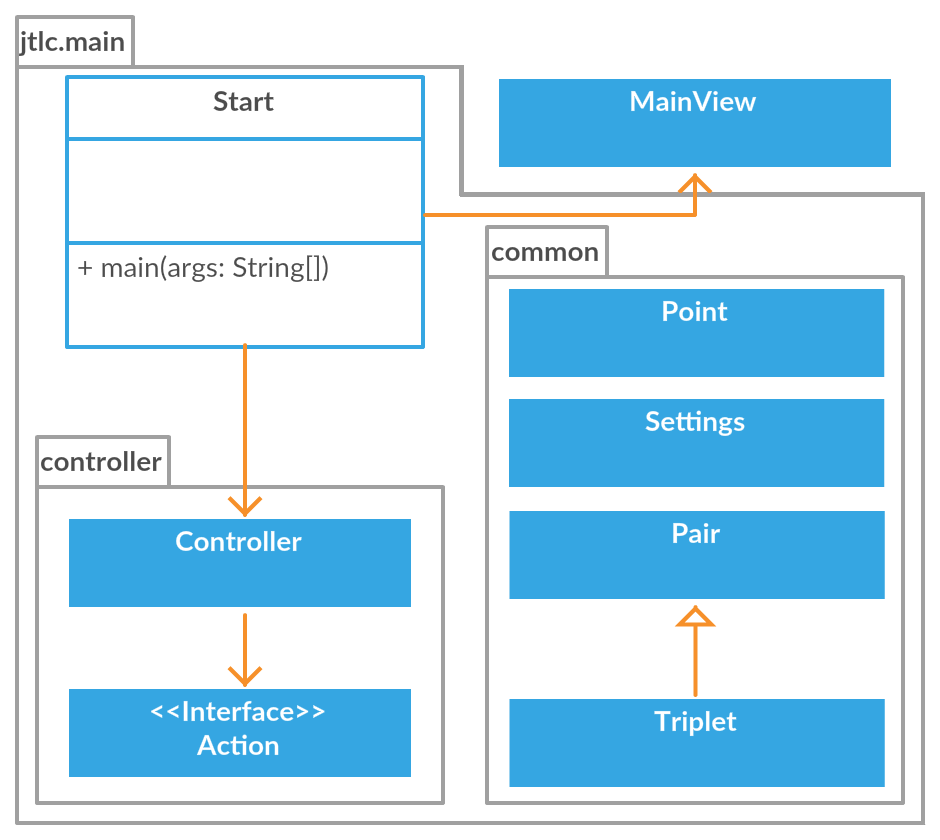
\includegraphics[width=325pt]{imagenes-jtlc/main}
	\centering
	\vspace{-0.5cm}
	\caption{Diagrama de Clases paquete \textit{jtlc.main}.}
	\label{fig:mainDiagrama}
\end{figure}

\begin{figure}[H]
	\centering
	\vspace{-0.5cm}
	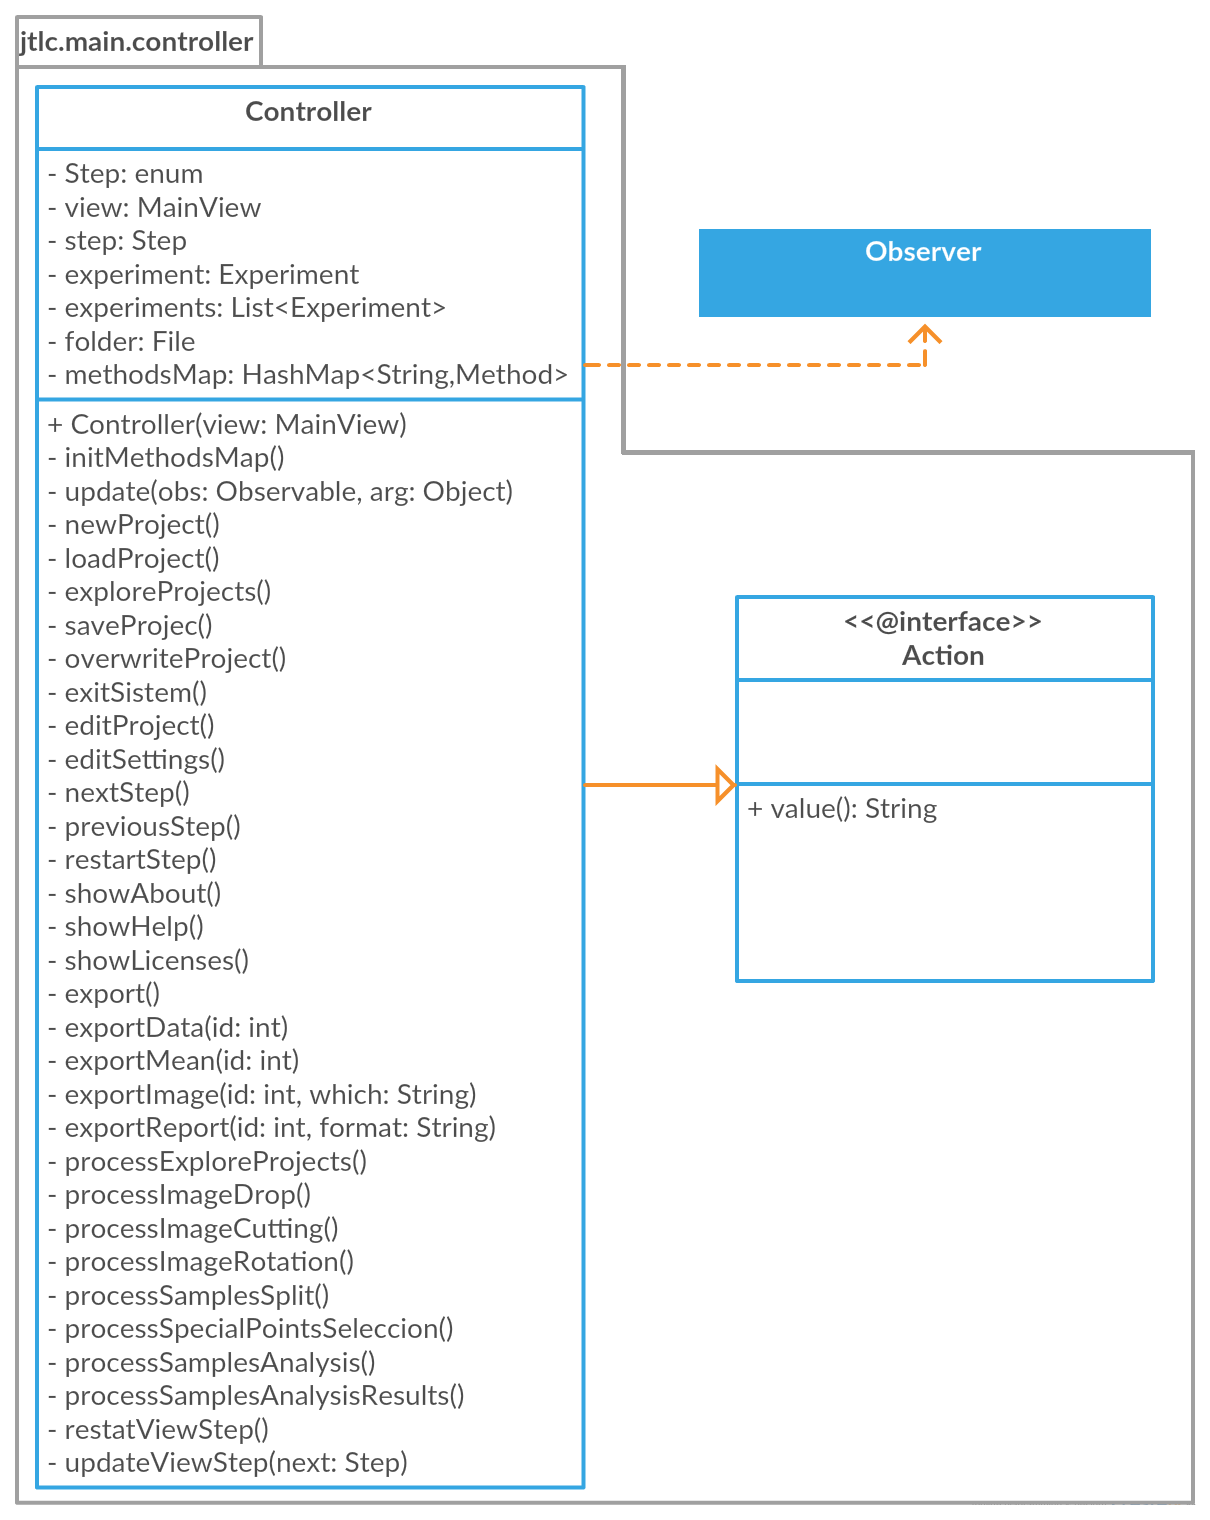
\includegraphics[width=425pt]{imagenes-jtlc/controller}
	\centering
	\vspace{-0.5cm}
	\caption{Diagrama de Clases paquete \textit{jtlc.main.controller}.}
	\label{fig:controllerDiagrama}
\end{figure}

\section{Prueba}
La prueba del sistema no se realiz\'o siguiendo ning\'un mecanismo sistem\'atico de testing (como por ejemplo, testing de unidad usando JUnit), s\'olo se realizaron pruebas \textit{Ad hoc} sin planificaci\'on ni documentaci\'on. Estas pruebas fueron llevadas a cabo corriendo el sistema, probando diferentes escenarios observando el comportamiento del mismo y contrast\'andolo con el esperado. En este caso se realizaron an\'alisis de muestras que fueron previamente analizadas usando otro \textit{software} y se compararon los resultados obtenidos con nuestro sistema contra los resultados obtenidos a partir de otro \textit{software} de an\'alisis cromatogr\'afico observando resultados bastante similares entre ambos con una tolerancia al error aceptable. Dada la naturaleza gr\'afica del problema y el asistente del proceso de an\'alisis, gran parte de las pruebas estuvieron concentradas en las funcionalidades provistas por las vistas y paneles los cuales fueron desarrolladas testeando su comportamiento y resultados, principalmente la alineaci\'on de los \textit{sliders} con las im\'agenes y el \textit{plotter} para garantizar la precisi\'on de los resultados y de las \'areas seleccionadas. Algunos problemas que surgieron a partir de las pruebas fueron de control de datos faltantes, por ejemplo, al momento de seleccionar las muestras individuales ocurr\'ia un error si se intentaba continuar el proceso sin haber seleccionado ninguna muestra, el cual fue f\'acilmente solucionado comprobando que la cantidad de muestras seleccionadas sea mayor a 0, mostrando una advertencia en caso de no ser as\'i sin poder continuar el proceso.\\
A partir de una versi\'on estable del sistema se desarrollo una etapa importante de las pruebas que consistieron en la aprobaci\'on del funcionamiento del sistema por parte del experto en el \'area \emph{Pablo Rossi} el cual junto a su equipo de trabajo actualmente utilizan la aplicaci\'on en un ambiente de producci\'on, ellos son los principales usuarios que reportaran posibles errores en el sistema o mejoras a desarrollar.
